%
% Szablon, v. 3.0
% p.wlaz@pollub.pl
%

% PROSZĘ NIE USUWAĆ
% KOMENTARZY Z~PREAMBUŁY
% JEŻELI KTOŚ WAM WMAWIA, ŻE
% TO PRZYSPIESZY COKOLWIEK
% -- MYLI SIĘ!


\documentclass[12pt]{mwbk}


%%%%%%% marinesy, rozmiary, to warto dopasować do drukarki
\usepackage[a4paper,twoside,top=2.6cm,bottom=2.6cm,inner=3cm,outer=2.6cm]{geometry}

%%%%%%%% polszczyzna
\usepackage[T1]{polski}


%%%%%%%%% sposób kodowania literek w edytorze
\usepackage[utf8]{inputenc}

\usepackage[font=small,labelfont=bf,justification=centering]{caption}


%%%% gdyby ktoś chciał powyklejać z~pedeefa
%%%% teksty za pomocą AcroReadera, to 
%%%% poniższe dwie linijki pomogą w~tym
%%%% Może to być przydatne, gdyby ktoś na podstawie
%%%% elektronicznej wersji chciał przygotować dane do 
%%%% badania antyplagiatowego
%%%% ponieważ prace są w
%%%% tych czasach różnymi
%%%% programami antyplagiatowymi
%%%% proszę absolutni NIE
%%%% USUWAĆ następujących
%%%% dwu linijek
\input glyphtounicode.tex
\pdfgentounicode = 1

%%%%%%%%%%%%%%%%%%%%%%%%%%%%%%%%%%%%%
%%%%% jeśli chcesz by główny tekst oraz wzory matematyczne były
%%%%% składane czcionką typu Times Roman (w~odróżnieniu od standardowej
%%%%% TeXowej, czyli Computer Modern Roman) to linia poniżej
%%%%% ma być 'aktywna', następna nieaktywna, 
%%%%% jeśli zrobisz odwrotnie (pierwsza nieaktywna,
%%%%% druga aktywna) uzyskasz skład czcionką
%%%%% Computer Modern Roman mającą wielu wiernych
%%%%% fanów w~świecie TeXa). Konsekwencją jednak będą zmiany
%%%%% rozmiarów czcionek dla rozdziałó i podrozdziałów - rzecz bez większego
%%%%% znaczenia, wynikająca z pewnych zaszłości historycznych (ComputerModern
%%%%% niegdyś były używane wyłącznie w postaci tzw. bitmap)
\usepackage{mathptmx} \usepackage{tgtermes}
%\usepackage{lmodern}

%%% WSZELKIE ZMIANY W~PREAMBULE RÓB ROZWAŻNIE
%%% NIE JESTEŚ PEWNY/PEWNA ICH EFEKTU TO~SPRAWDŹ 
%%% CZY W~PRGRAMIE ADOBE READER (i~to dokładnie
%%% o~ten program chodzi, nie o~jakikolwiek)
%%% Z~WYNIKOWEGO PLIU PDF DA SIE PRAWIDŁOWO
%%% WYKLEIĆ TEKST Z~POLSKIMI LITERAMI, BEZ KRZAKÓW,
%%%% BEZ DZIWACTW.


%%%%%%%%%%%%%% pozostałe pakiety używane w~pracy, to już zależy od
%%%%%%%%%%%%%% autora, więc może być tego więcej
\usepackage{fancyhdr}
\usepackage{graphicx}
\usepackage{amsmath}
\usepackage{amsthm}
\usepackage{amssymb}
\usepackage{url}
\usepackage{longtable}
\usepackage{array,hhline}

%%%%%%%% hyperref po to by przeglądarka pedeef ukazywala na odwołania
%%%%%%%% prawidłowo skonstruowane za pomocą \ref, \cite i.t.d. jako
%%%%%%%% hiperłącza
\usepackage{hyperref}



%%%%% dla fanów ``profesjonalnych'' tabel w~stylu zachodnich książek

\usepackage{booktabs} \heavyrulewidth=1.5bp \lightrulewidth=0.5bp


%%%%%%%%%%% poniżej uniwersalny sposób na ucywilizowanie znaków 
%%%%%%%%%%% niewiększości, niezależny od pakietu {polski}, ale za to 
%%%%%%%%%%% zależny od {amssymb}, ma tą zaletę, że działa np. z Timesem
%%%%%%%%%%% w matematyce
\let\leq\leqslant\let\le\leq\let\geq\geqslant\let\ge\geq


%%%%%%% jeżeli będziesz chciał włączać do swojej pracy fragmenty programów, 
%% to ponizsza linijka przyda się, jeśli nie - usuń ją

\usepackage{fancyvrb}


%%%%%%%%%%%%%%%%% struktury do tworzenia twierdzeń i~tym podobnych

\theoremstyle{plain}
\newtheorem{twier}{Twierdzenie}[chapter] % pierwsze to nazwa środowiska,
                                      %drugie to wyświetlana nazwa
				% to trzecie w~nawiasie kwadratowym
				% wskazuje numer dolepiony z~lewej do
				% numeru twierdzenia (tu numer
				% 'chapter', 
\newtheorem{lemat}{Lemat}[chapter]

\theoremstyle{definition}
\newtheorem{defi}{Definicja}[chapter]

\theoremstyle{remark}
\newtheorem{uwaga}{Uwaga}[chapter]
\newtheorem{wniosek}{Wniosek}[chapter]

%%%%% więcej możliwości w~dokumentacji amsthm



%%%%%%%%%%%%%%%%%%%%%%%%%%%%%%%%%%%%%%%%%5
%%%%%%%%%%%%%%%%%%%%%%%%%%%%%%%%%%%%%%%%%%
%%%%%%%%% wcięcie akapitowe %%%%%%%%%%%%%%
%%%%%%%%%%%%%%%%%%%%%%%%%%%%%%%%%%%%%%%%%%
%%%%%% ustawić w~zaleceń i~gustu %%%%%%%%%
%%%%%%%%%%%%%%%%%%%%%%%%%%%%%%%%%%%%%%%%%%
%%%%%%%% zalecenie na stronie wydziałowej
%%%%%%%% było 1.25cm i wyglądało jakoś 
%%%%%%%% śmiesznie duże, więc spłoszony nieco
%%%%%%%% wpisałem 1cm, ale uważny czytelnik już
%%%%%%%% zapewne się domyśli, że podmiana napisu 
%%%%%%%% =1cm na =1.25cm sprawi, że wcięcia na początku
%%%%%%%% akapitu ustawią się na (nieco przydużą)
%%%%%%%% wartość 1.25cm 

\parindent=1cm



%%%%%%%%%%%%%%%%%%%%%%%%%%%%%%%%
%%%%% tu pewne poluzowanie rozmieszczenia elementów tabelek
%%%%% możecie sobie poeksperymentować, by dopasować do swych
%%%%% gustów, a przede wszystkim gustów promotorów (promotorek)
  \tabcolsep=4mm          
  %\renewcommand\arraystretch{1.3}
%%%%%%%%%%%%%%%%%%%%%%%%%%%%%%%%%%



%%%%%%%%% teraz żywa pagina (aka 'running headline') i~numerowanie stron
%%%%%%%%%%%%%%%%%%%%%%%%%%%%%%%%%%%%%%%%%%%%%%%%%%%%%%%%%%%%%%%%%%%%%%%%
%%%%%na górze mają być śródtytuły, na dole (po stronie zewneętrznej)
%%%%%numery stron. Poszedłem kapkę dalej i~na stronach ropoczynających
%%%%%rozdział nie ma paginy (górki).
%%%%% Oczywiście jeśli ostatnia strona
%%%%% jest pusta (uzupełnia jeno parzystość) to tam żadnej stopki ani 
%%%%% górki byc mnie może - ma być pusta.
%%%%%%%%%%%%%%%%%%%%%%%%%%%%
\pagestyle{fancy}
\fancyhead{}% oczyszczenie
\fancyhead[RO]{\rightmark} %% na nieparzystych 'podległe' śródtytuły
\fancyhead[LE]{\leftmark} %% na parzystych 'ważniejsze'
\fancyfoot{}% oczyszczenie
\fancyfoot[RO,LE]{\arabic{page}}  %% numer na dole (po prawej na
%% nieparzystych, po lewej na parzystych)
\renewcommand\headrulewidth{0.4pt} %%% cienka hrulka oddzielająca paginę
                                    %%% od kolumny tekstu
\fancypagestyle{closing}{%%%%%% to styl dla stron zamykających rozdział
\fancyhead{}% oczyszczenie
\fancyhead[RO]{\rightmark} %% na nieparzystych 'podległe'
\fancyhead[LE]{\leftmark} %% na parzystych 'ważniejsze'
\fancyfoot{}% oczyszczenie
\fancyfoot[RO,LE]{\arabic{page}}  %% numer na dole (po prawej na
                                  %% powyższą linijkę usuń jeśli nie
				  %% chcesz numerów na niepełnych
				  %% kolumnach (zamykających rozdział)
\renewcommand\headrulewidth{0.4pt}
}
\fancypagestyle{opening}{%%% styl stron rozpoczynających rozdział
\fancyhead{}% oczyszczenie
\fancyfoot{}% oczyszczenie
\fancyfoot[RO,LE]{\arabic{page}}  %% numer na dole (po prawej na
\renewcommand\headrulewidth{0pt}
}
\fancypagestyle{plain}{%%%% styl zwykły, niektóre konstrukcje
                       %%%% (typu \titlepage, którego ja tu nie używam
                       %%%% ale może są jakieś inne o których nawet nie chce 
                       %%% mi się myśleć, więc dla spokoju robię to po swojemu
\fancyhead{}% oczyszczenie
\fancyfoot{}% oczyszczenie
\fancyfoot[RO,LE]{\arabic{page}}  %% numer na dole (po prawej na
\renewcommand\headrulewidth{0pt}
}

%%%%%%%%%%%%%%%%%%%%%%%%%%%%%%%%%5
%%%%%%%%%%%%%%%%%%%%%%%%%%%%%%%%%%
%%% lekka modyfikcja 'markow' do paginy
%%% uznalem, ze jesli ktos nie da \section (np we wstepnie czy
%%% podsumowaniu to niech na obu sronach w~paginie pojawia sie tytuł
%%% chaptera, bo standardowo, to na nieparzystej stronie w takiej sytuacji
%%% nad górną linią ziałaby pustka, co mogłoby wprowadzać konsternację
\makeatletter
    \def\chaptermark#1{%
      \markboth{%
        \ifHeadingNumbered
     \if@mainmatter
     \@chapapp\
            \thechapter.\enspace
          \fi
        \fi
        #1}{%
        \ifHeadingNumbered
     \if@mainmatter
     \@chapapp\
            \thechapter.\enspace
          \fi
        \fi
        #1%
	}}%
    \def\sectionmark#1{%
      \markright{%
        \ifHeadingNumbered \thesection.\enspace \fi
        #1}}
%%%%%%%%%%%%%%%%%%%%%%%%%%%%%%%%%%%%%%%%%%%%%%%
%%%%%%%%%%%%%%%%%%%%%%%%%%%%%%%%%%%%%%%%%%%%%%%%
%%%%%%%%%%%% wielkości czcionek dla chapter i~section
%%%%%%%%%%%% 16 dla rozdziału, 14 dla podrozdziału - te domyślne
%%%%%%%%%%%% w klasie mwbk były całkiem ładne, ale żeby nie było
%%%%%%%%%%%% że nie potrafię ustawić
%%%%%%%%%%%%%%%%%%%%%%%%%%%%%%%%%%%%%%%%%%%%%%%%%%%
\SetSectionFormatting[breakbefore,wholewidth]{chapter}
        {0\p@}
        {\FormatRigidChapterHeading{6.4\baselineskip}{12\p@}%
	{\large\@chapapp\space}{\fontsize{16}{19}\selectfont}}
        {1.6\baselineskip}
\SetSectionFormatting{section}
        {24\p@\@plus5\p@\@minus2\p@}
	{\FormatHangHeading{\fontsize{14}{16}\selectfont}}
        {10\p@\@plus3\p@}
\makeatother	



%%%%%%%%%%%%%%%%%%%%%%%%%%%%%%%%%%%%%%%%%%%%%%
%%%%%%%%%%%%%%%%%%%%%%%%%%%%%%%%%%%%%%%%%%%%%%
%%%%%%%%%%%%%% jakies inne pomocnicze definicje, ja na przykład lubię
% \R
%%%%%%%%%%%%%%%%%%%%%%%5
%%%%%%%%%%%%%%%%%%%%%%%
%%%% tak naprawdę są t potrzebne tylko po to
%%%% by zadziałały przykłady poniżej w tekście
%%%% które w sposób dość losowy zostały 
%%%% pobrane z jakichś moich starych plików
%%%%%%%%%%%%%%%%%%%%%%%%%%%%%%%%%%
%%%%%%%%%%%%%%%%%%%%%%%%%%%%%%%%%%%
%%%% w realnej pracy te poniższe śmieci możecie oczywiście
%%%% usunąć
%%%%%%%%%%%%%%%%%%%%%%%%%%%%
\newcommand\R{\mathbb{R}}
\newcommand{\ff}{\mathbf{f}}
\newcommand{\hh}{\mathbf{h}}
\newcommand{\xx}{\mathbf{x}}
\newcommand{\yy}{\mathbf{y}}
\newcommand{\zz}{\mathbf{z}}
\newcommand{\gggg}{\mathbf{g}}
\newcommand{\skalar}[2]{\pmb{\langle}#1,#2\pmb{\rangle}}
%%%%%%%%%%%% koniec tych dodatkowych definicji

%%%%%% trocę więcej ``luzu'' przy rozmieszczaniu {fgur} i~{table}

 \renewcommand{\topfraction}{0.9}	% max fraction of floats at top
    \renewcommand{\bottomfraction}{0.8}	% max fraction of floats at bottom
    %   Parameters for TEXT pages (not float pages):
    \setcounter{topnumber}{2}
    \setcounter{bottomnumber}{2}
    \setcounter{totalnumber}{4}     % 2 may work better
    \setcounter{dbltopnumber}{2}    % for 2-column pages
    \renewcommand{\dbltopfraction}{0.9}	% fit big float above 2-col. text
    \renewcommand{\textfraction}{0.07}	% allow minimal text w. figs
    %   Parameters for FLOAT pages (not text pages):
    \renewcommand{\floatpagefraction}{0.7}	% require fuller float pages
    % N.B.: floatpagefraction MUST be less than topfraction !!
    \renewcommand{\dblfloatpagefraction}{0.7}	% require fuller float pages
    % remember to use [htp] or [htpb] for placement

    
%%% DWA proste polecenia służące do ujednolicenia podawania źródeł przy rysunkach i~tabelkach    
    
    \newcommand\zrodlo[1]{\par\vspace{-3mm}{\small\textit{Źródło: }#1 }}
    \newcommand\zrodlotab[1]{{\par\vspace{2mm}\small\textit{Źródło: }#1 }}

\raggedbottom   %%% to znaczy, że nie będzie siłowego wyrównywania typowych
                %%     stron do jednakowej wysokości

\linespread{1.3}
\begin{document}

%%%%%%%%%%%%%%%%%%%%%%%%%%%%%%%%%%%%%%%%%
%%%%%%%%%%%%%%%%%%%%%%%%%%%%%%%%%%%%%%%%%
%%%%%%%% STRONA TYTUŁOWA %%%%%%%%%%%%%%%%

\thispagestyle{empty}  % tu wszak nie chcemy żadnej numeracji stron


%%%%%%%%%%%%%%%%%%%%%%%%%%%%%%%%%%%%%%%%%%%%%%%%%%%%%%%%%%%%%%%
%%%%%tytuły definiuje jako makrodefinicje, gdyż zamierzam je%%%
%%%%%powtórzyć na stronie ze streszczeniami, to nic nie boli%%%
%%%%%a gwarantuje, że będą one takie same, i~tak ma być.%%%%%%%
%%%%%%%%%%%%%%%%%%%%%%%%%%%%%%%%%%%%%%%%%%%%%%%%%%%%%%%%%%%%%%%
\newcommand\tytul{Przegląd autoenkoderów stosowanych w nienadzorowanym uczeniu maszynowym}

\newcommand\tytulangielski{An overview of autoencoders used in unsupervised machine learning}



\noindent\hspace{-32pt}
\includegraphics{rys/logopl}
\begin{center}
	



%%{\large \bf POLITECHNIKA LUBELSKA}

%%%% {\bf WYDZIAŁ PODSTAW TECHNIKI} tego już nie chcą w~nowym wzorcu karty

%%%% \emph{Kierunek:} MATEMATYKA   %% już jest w~``logo''

%%% BEZ SPEC.!!! \emph{Specjalność:} Matematyka w~finansach i~ubezpieczeniach

\vfill %%%% \vfill to taki rozpychacz w pionie, pcha ile mu pozwolą
     


\vfill

\textbf{Praca magisterska}

\vfill
\vfill
\vfill

\large
\tytul

\vfill

\emph{\tytulangielski}


\vfill
\vfill
\vfill
\vfill
\vfill

\begin{tabular}[t]{l}
\emph{Praca wykonana pod kierunkiem:}
\\
dra Dariusza Majerka
\end{tabular}
\hfill
\begin{tabular}[t]{l}
	\emph{Autor:}
\\
Alicja Hołowiecka\\
nr albumu: 89892 
\end{tabular}

\vfill
\vfill
\vfill

\textbf{Lublin 2022}

\end{center}


%%%%% koniec tytułów


%%%%%%%%%%%%%%%%%%%%%%%5
%%%%%%%%%%%%%%%%%%%%%%
%%% teraz spis treści
%%%%%%%%%%%%%%%%%%%%%
%%% pamiętaj! po jakiejkolwiek zmianie w tekście
%%% która wpływa na zmianę spisu treści, spis będzie dobry co najmniej
%%% po dwóch przebiegach latexa - to samo dotyczy odwołań do wzorów i literatury
%%% ogólnie to przed wydrukiem warto przelatexować o jedne raz więcej niż
%%% to się wydaje konieczne, no chyba że korzystamy z funkcji typu BUILD
%%% w zintegrowanym systemie wspomagającym TeX, BUILD powinien takie sprawy 
%%% wziąć pod uwagę

\tableofcontents


\chapter*{Wstęp}



\chapter{Przegląd autoenkoderów}

\section{Sztuczne sieci neuronowe}

\textbf{Sztuczny neuron} jest systemem składającym się z co najmniej jednego binarnego wejścia i dokładnie jednego binarnego wyjścia. Wyjście uaktywnia się, jeżeli jest aktywna określona liczba wejść. Sztuczne neurony są podstawowym elementem sztucznych sieci neuronowych. Do pewnego stopnia są inspirowane budową biologicznego neuronu. Na rysunku \ref{fig:neurony1} przedstawione są przykładowe sztuczne sieci neuronowe (SSN lub z angielskiego ANN) wykonujące różne operacje logiczne. W tych przykładach przyjęto, że neuron uaktywni się, gdy przynajmniej dwa wejścia będą aktywne \cite{geron}.

\begin{figure}[!h]
	\centering
	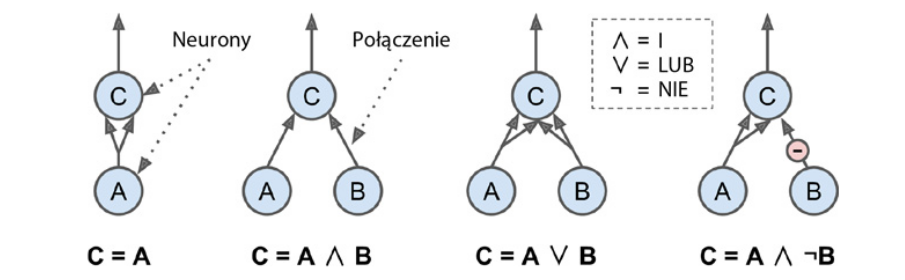
\includegraphics[width=9cm]{rys/neurony1.png}
	\caption{Przykładowe sztuczne sieci neuronowe rozwiązujące proste zadania logiczne}
	\zrodlo{\cite{geron}}
	\label{fig:neurony1}
\end{figure}

Jedną z najprostszych architektur SSN jest \textbf{perceptron}, którego podstawą jest sztuczny neuron zwany \textbf{progową jednostką logiczną} (ang. \textit{Threshold Logic Unit} - TLU) lub \textbf{liniową jednostką progową} (ang. \textit{Linear Threshold Unit} - LTU). Wartościami wejść i wyjść są liczby, a każde połączenie ma przyporządkowaną wagę. Jednostka TLU oblicza ważoną sumę sygnałów wejściowych, a następnie zostaje użyta funkcja skokowa na tej sumie. Schemat takiej jednostki został przedstawiony na rysunku \ref{fig:neurony2}.
\begin{figure}[!h]
	\centering
	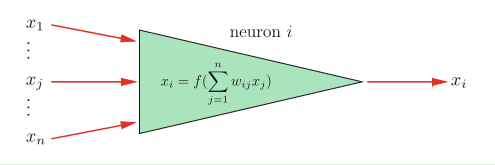
\includegraphics[width=8cm]{rys/neurony2.png}
	\caption{Struktura sztucznego neuronu, który stosuje funkcję skokową $f$ na ważonej sumie sygnałów wejściowych}
	\zrodlo{\cite{ertel}}
	\label{fig:neurony2}
\end{figure}
Często używaną funkcją skokową jest \textbf{funkcja Heaviside'a}, określona równaniem 
$$H(z)=\begin{cases}
0, & \text{ jeśli } z<0\\
1, & \text{ jeśli } z \geq 0
\end{cases}$$
Czasami zamiast niej stosuje się również \textbf{funkcję signum}:
$$sgn(z)=\begin{cases}
-1 & \text{ jeśli } z<0\\
0, & \text{ jeśli } z=0\\
1, & \text{ jeśli } z > 0
\end{cases}$$

Perceptron jest złożony z jednej warstwy jednostek TLU, w której każdy neuron jest połączony ze wszystkimi wejściami. Warstwa tego typu nazywana jest \textbf{warstwą gęstą}. Warstwa, do której są dostarczane dane wejściowe, jest nazywana \textbf{warstwą wejściową} (ang. \textit{input layer}). Najczęściej do tej warstwy jest wstawiany również \textbf{neuron obciążeniowy} (ang. \textit{bias neuron}) $x_0=1$, który zawsze wysyła wartość 1. Na rysunku \ref{fig:perceptron1} znajduje się perceptron z dwoma neuronami wejściowymi i jednym obciążeniowym, a także z trzema neuronami w warstwie wyjściowej.

\begin{figure}[!h]
	\centering
	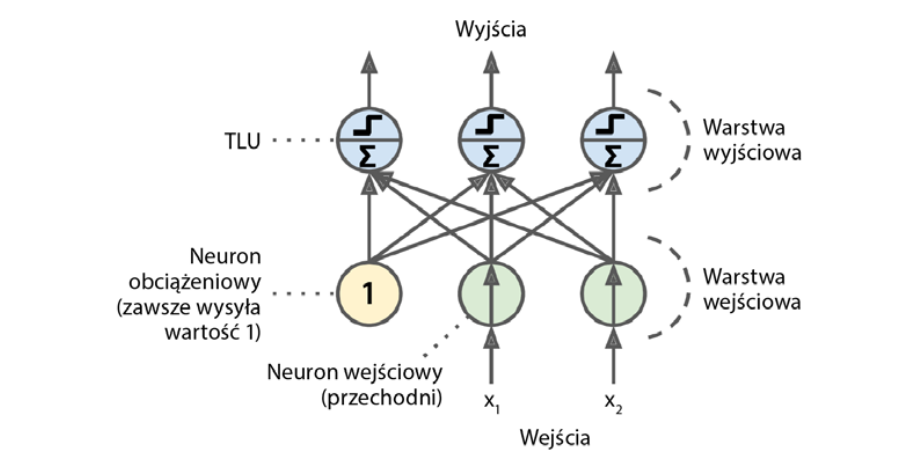
\includegraphics[width=10cm]{rys/perceptron1.png}
	\caption{Perceptron z trzema neuronami wejściowymi i trzema wyjściami}
	\zrodlo{\cite{geron}}
	\label{fig:perceptron1}
\end{figure}

Obliczanie sygnałów wyjściowych w warstwie gęstej przedstawia się wzorem
$$h_{\mathbf{W},\mathbf{b}}(\mathbf{X})=\phi(\mathbf{XW}+\mathbf{b})$$
gdzie $\mathbf{X}$ - macierz cech wejściowych, $\mathbf{W}$ - macierz wag połączeń (oprócz neuronu obciążeniowego), $\mathbf{b}$ - wektor obciążeń zawierający wagi połączeń neuronu obciążeniowego ze wszystkimi innymi neuronami, $\phi$ - tzw. \textbf{funkcja aktywacji}, w przypadku TLU jest to funkcja skokowa.

Algorytm uczący, który służy do trenowania perceptronu, jest silnie inspirowany działaniem neuronu biologicznego. Gdy biologiczny neuron często pobudza inną komórkę nerwową, to połączenia między nimi stają się silniejsze. Reguła ta jest nazywana \textbf{regułą Hebba}. Perceptrony są uczone za pomocą odmiany tej reguły, w której połączenia są wzmacniane, jeśli pomagają zmniejszyć wartość błędu. Dokładniej, w danym momencie perceptron przetwarza jeden przykład uczący i wylicza dla niego predykcję. Na każdy neuron wyjściowy odpowiadający za nieprawidłową prognozę następuje zwiększenie wag połączeń ze wszystkimi wejściami przyczyniającymi się do właściwej prognozy. Aktualizowanie wag przedstawia się następującym wzorem
$$\Delta w_{ij}=\eta (y_j-\hat{y_j})x_i$$
gdzie $w_{ij}$ - waga połączenia między $i$-tym neuronem wejściowym a $j$-tym neuronem wyjściowym, $x_i$ - $i$-ta wartość wejściowa bieżącego przykładu uczącego, $\hat{y_j}$ - wynik $j$-tego neuronu wyjściowego dla bieżącego przykładu uczącego, $y_j$ - docelowy wynik $j$-tego neuronu, $\eta$ - współczynnik uczenia.

Perceptron ma wiele wad związanych z niemożnością rozwiązania pewnych trywialnych problemów (np. zadanie klasyfikacji rozłącznej czyli XOR). Część tych ograniczeń można wyeliminować, stosując architekturę SSN złożoną z wielu warstw perceptronów, czyli \textbf{perceptron wielowarstwowy} (ang. \emph{Multi-Layer Perceptron}). Składa się on z jednej warstwy wejściowej (przechodniej), co najmniej jednej warstwy jednostek TLU - tzw. \textbf{warstwy ukryte} (ang. \emph{latent layers}) i ostatniej warstwy jednostek TLU - warstwy wyjściowej. Oprócz warstwy wejściowej każda warstwa zawiera neuron obciążający i jest w pełni połączona z następną wartswą. Sieć zawierająca wiele warstw ukrytych nazywamy \textbf{głęboką siecią neuronową} (ang. \emph{Deep Neural Network} - DNN). 

Do uczenia perceptronów wielowarstwowych wykorzystywany jest algorytm \textbf{propagacji wstecznej} (ang. \emph{backpropagation}). Propagacja wsteczna jest właściwie algorytmem gradientu prostego \cite{skansi}. Można go zapisać jako
$$w_{updated}=w_{old}-\eta \nabla E$$
gdzie $E$ jest funkcją kosztu (funkcją straty) \cite{skansi}. Proces jest powtarzany do momentu uzyskania zbieżności z rozwiązaniem, a każdy przebieg jest nazywany \textbf{epoką} (ang. \emph{epoch}).

\begin{uwaga}
	Wagi połączeń wszystkich warstw ukrytych należy koniecznie zainicjować losowo. W przeciwnym przypadku proces uczenia zakończy się niepowodzeniem. Na przykład jeśli wszystkie wagi i obciążenia zostaną zainicjowane wartością 0, to model będzie działał tak, jak gdyby składał się tylko z jednego neuronu. Przy zainicjowaniu wag losowo, symetria zostanie złamana i algorytm propagacji wstecznej będzie w stanie wytrenować zespół zróżnicowanych neuronów \cite{geron}. 
\end{uwaga}

Aby algorytm propagacji wstecznej działał prawidłowo, kluczową zmianą jest zastąpienie funkcji skokowej przez inne \textbf{funkcje aktywacji}. Zmiana ta jest konieczna, ponieważ funkcja skokowa zawiera jedynie płaskie segmenty i przez to nie pozwala korzystać z gradientu. 

Najczęściej używana jest \textbf{funkcja logistyczna (sigmoidalna)}
$$\sigma(z)=\frac{1}{1+e^{-z}}$$
Ma ona w każdym punkcie zdefiniowaną pochodną niezerową, dzięki czemu algorytm gradientu prostego może na każdym etapie uzyskać lepsze wyniki. Zbiór wartości tej funkcji wynosi od 0 do 1.

Inną popularną funkcją aktywacji jest \textbf{tangens hiperboliczny}
$$\operatorname{tanh}(z)=2\sigma(2z)-1$$
Funkcja ta jest ciągła i różniczkowalna, a jej zakres wartości wynosi $-1$ do 1. Dzięki temu zakresowi wartości wynik każdej warstwy jest wyśrodkowany wobec zera na początku uczenia, co często pomaga w szybszym uzyskaniu zbieżności.

Wśród popularnych funkcji aktywacji należy także wyróżnić  \textbf{funkcję ReLU} (ang. \emph{Rectified Linear Unit} - prostowana jednostka liniowa) o wzorze
$$ReLU(z)=max(0,z).$$
Jest ona ciągła, ale nieróżniczkowalna w punkcie 0. Jej pochodna dla $z<0$ wynosi zero. Jej atutem jest szybkość przetwarzania. Nie ma ona maksymalnej wartości wyjściowej.
W zadaniach regresji bywa wykorzystywany ,,wygładzony'' wariant funkcji ReLU, czyli funkcja \textbf{softplus}:
$$softplus(z)=log(1+exp(z))$$

Na  rysunku \ref{fig:funkcje-aktywacji} przedstawiono popularne funkcje aktywacji wraz z ich pochodnymi.

\begin{figure}[!h]
	\centering
	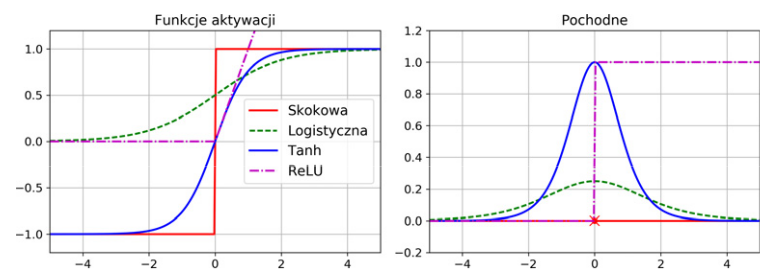
\includegraphics[width=\linewidth]{rys/funkcje_aktywacji.png}
	\caption{Przykładowe funkcje aktywacji wraz z pochodnymi}
	\zrodlo{\cite{geron}}
	\label{fig:funkcje-aktywacji}
\end{figure}


\newpage
\section{Sieci splotowe}


\subsection{Czym jest sieć splotowa}

\textbf{Splotowe sieci neuronowe} (ang. \emph{convolutional neural networks}, CNN) są rodzajem sieci neuronowych służących do przetwarzania danych o znanej topologii siatki. Przykładem takich danych są szeregi czasowe, które można uznać za jednowymiarową siatkę z próbkami w regularnych odstępach czasu, oraz dane graficzne, które można interpretować jako dwuwymiarową siatkę pikseli. Nazwa sieci splotowych pochodzi od wykorzystywanego przez te sieci działania matematycznego nazywanego \textbf{splotem} (konwolucją). Można powiedzieć, że sieci splotowe to po prostu sieci neuronowe, które w przynajmniej jednej z warstw zamiast ogólnego mnożenia macierzy wykorzystują splot \cite{goodfellow}.
Splotowe sieci neuronowe stanowią wynik badań nad korą wzrokową. Od lat 80-tych XX wieku są używane głównie rozpoznawania obrazów, w zagadnieniach takich jak klasyfikacja, detekcja obrazów, transfer stylu. Stanowią podstawę usług takich jak wyszukiwanie obrazu, inteligentne samochody, automatyczne systemy klasyfikowania filmów. Są skuteczne również w innych dziedzinach niż jedynie komputerowe widzenie - takie dziedziny to na przykład rozpoznawanie mowy (\emph{voice recognition}) oraz przetwarzanie języka naturalnego (\emph{Natural Language Processing, NLP}) \cite{geron}. 

%\subsection{Działanie kory wzrokowej}

Ponieważ splotowe sieci neuronowe są silnie inspirowane działaniem biologicznej kory wzrokowej, to ten podrozdział zostanie poświęcony wyjaśnieniu jej działania. Na podstawie badań prowadzonych pod koniec lat 50-tych XX wieku \cite{hubel1} \cite{hubel2} wykazano, że neurony biologiczne w korze wzrokowej reagują na określone wzorce w niewielkich obszarach pola wzrokowego, zwanych \textbf{polami recepcyjnymi}, a w miarę przepływu sygnału wzrokowego przez kolejne moduły w mózgu neurony rozpoznają coraz bardziej skomplikowane wzorce wykrywane w coraz większych polach recepcyjnych.
Wiele neuronów stanowiących korę wzrokową tworzy \textbf{lokalne pola recepcyjne}, reagujące jedynie na bodźce wzrokowe mieszczące się w określonym rejonie pola wzrokowego, przy czym lokalne pola recepcyjne poszczególnych neuronów mogą się na siebie nakładać. Takie pola recepcyjne łącznie tworzą całe pole wzrokowe. Dodatkowo badacze zauważyli, iż pewne neurony reagują wyłącznie na obrazy składające się z linii poziomych, lub innych linii ułożonych w konkretny sposób (dwa neurony mogą nawet mieć to samo pole recepcyjne, ale reagować na różne ułożenie linii). Badacze stwierdzili, że niektóre komórki nerwowe mają większe pola recepcyjne i wykrywają bardziej skomplikowane kształty. Takie neurony, odpowiedzialne za rozpoznawanie bardziej skomplikowanych kształtów, znajdują się na wyjściu neuronów reagujących na prostsze bodźce. Działanie neuronów biologicznych w korze wzrokowej, zgodnie z powyższym opisem, zostało zobrazowane na rysunku \ref{fig:kora-wzrokowa}.


\begin{figure}[!h]
	\centering
	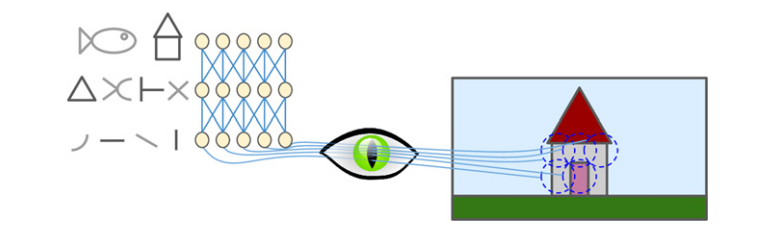
\includegraphics[width=\linewidth]{rys/kora_wzrokowa.png}
	\caption{Działanie neuronów biologicznych w korze wzrokowej}
	\zrodlo{\cite{geron}}
	\label{fig:kora-wzrokowa}
\end{figure}

\subsection{Elementy sieci splotowej}

\subsubsection{Warstwy splotowe}

Przejdziemy teraz do opisu najistotniejszej części sieci CNN, jaką jest warstwa splotowa (\emph{convolutional layer}). Na rysunku \ref{fig:warstwy-cnn} widoczny jest przykład warstw splotowych z prostokątnymi polami recepcyjnymi. W pierwszej warstwie splotowej, neurony nie są połączone z każdym pikselem obrazu wejściowego (w przeciwieństwie do opisanych wcześniej warstw gęstych), lecz jedynie z pikselami znajdującymi się w polu recepcyjnym danego neuronu. W kolejnej warstwie każdy neuron łączy się wyłącznie z neuronami z niewielkiego obszaru pierwszej warstwy. Dzięki temu sieć koncentruje się na pewnych cechach w pierwszej warstwie, a w drugiej warstwie może je łączyć w bardziej złożone kształty. Taka hierarchiczna struktura w naturalny sposób występuje na zdjęciach, co przyczyniło się do dużej skuteczności sieci splotowych w rozpoznawaniu obrazu.

\begin{figure}[!h]
	\centering
	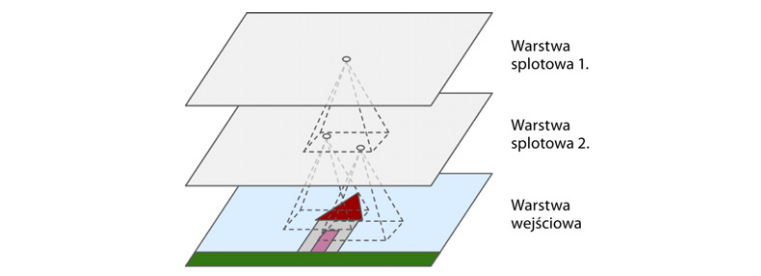
\includegraphics[width=\linewidth]{rys/warstwy_cnn.png}
	\caption{Warstwy splotowe z prostokątnymi lokalnymi polami recepcyjnymi}
	\zrodlo{\cite{geron}}
	\label{fig:warstwy-cnn}
\end{figure}

Neuron znajdujący się w wierszu $i$ oraz kolumnie $j$ danej warstwy jest połączony z wyjściami neuronów poprzedniej warstwy zlokalizowanymi w rzędach od $i$ do $i+f_h -1$ i kolumnach od $j$ do $j+f_w -1$,
gdzie $f_h$ i $f_w$ oznaczają, odpowiednio, wysokość i szerokość pola recepcyjnego (rysunek \ref{fig:zero-padding}). W celu
uzyskania takich samych wymiarów każdej warstwy najczęściej są dodawane zera wokół wejść, co zostało pokazane na rysunku \ref{fig:zero-padding}. Proces ten nazywamy \textbf{uzupełnianiem zerami} (ang. zero padding).

\begin{uwaga}[Dopełnianie]
	Dopełnianie (padding) jest ściśle związane z parametrem kroku (który zostanie opisany w kolejnym akapicie). Zapewnia poprawność obliczeń w warstwie konwolucyjnej \cite{illustrated}.
\end{uwaga}

\begin{figure}[!h]
	\centering
	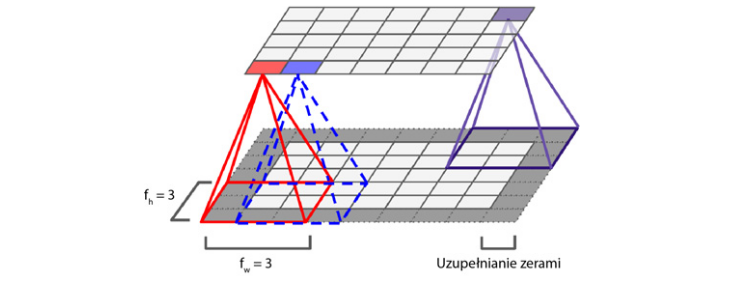
\includegraphics[width=\linewidth]{rys/zero_padding.png}
	\caption{Związek pomiędzy warstwami a uzupełnianiem zerami}
	\zrodlo{\cite{geron}}
	\label{fig:zero-padding}
\end{figure}

Możliwe jest również łączenie bardzo dużej warstwy wejściowej ze znacznie mniejszą kolejną warstwą
poprzez rozdzielanie pól recepcyjnych, tak jak zaprezentowano na rysunku \ref{fig:stride}. Rozwiązanie to
zmniejsza drastycznie złożoność obliczeniową modelu. Odległość pomiędzy dwoma kolejnymi polami
recepcyjnymi nosi nazwę \textbf{kroku} (ang. stride). Na widocznym schemacie warstwa wejściowa o wymiarach 5×7 (plus uzupełnianie zerami) łączy się z warstwą o rozmiarze 3×4 za pomocą pól recepcyjnych będących kwadratami 3×3 i kroku o wartości 2 (w omawianym przykładzie krok jest taki sam w obydwu wymiarach, ale nie jest to wcale regułą). Neuron zlokalizowany w rzędzie $i$ oraz kolumnie $j$ górnej warstwy łączy się z wyjściami neuronów dolnej warstwy mieszczącymi się w rzędach od $i\times s_h$ do $i\times s_h +f_h -1$ i w kolumnach od $j\times s_w$ do $j \times s_w +f_w -1$, gdzie $s_h$ i $s_w$ definiują wartości kroków odpowiednio w kolumnach i rzędach.


\begin{figure}[!h]
	\centering
	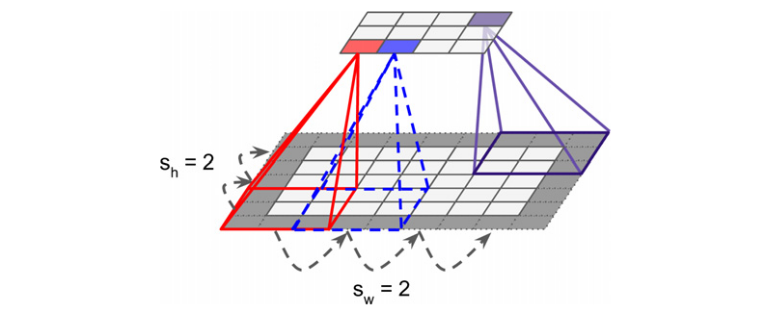
\includegraphics[width=0.9\linewidth]{rys/cnn_stride.png}
	\caption{Warstwa splotowa z krokiem o długości 2}
	\zrodlo{\cite{geron}}
	\label{fig:stride}
\end{figure}

\begin{uwaga}[Długość kroku]
	Długość kroku (stride length) - oznacza odległość, o jaką jądro przesuwa się po obrazie. Często stosowaną wielkością jest długość jednego piksela. Często wybieraną długością są również dwa piksele, rzadziej trzy. Dłuższe kroki nie są stosowane, ponieważ jądro może wtedy pomijać obszary obrazu potencjalnie wartościowe dla modelu. Z drugiej strony, im dłuższy krok, tym większa szybkość uczenia się modelu, ponieważ jest mniej obliczeń do wykonania. Trzeba znajdować kompromis między tymi efektami \cite{illustrated}.
\end{uwaga}

\subsubsection{Filtry}

Wagi neuronu mogą być przedstawiane jako niewielki obraz o rozmiarze pola recepcyjnego. Na
przykład na rysunku \ref{fig:filtry} widzimy dwa możliwe zbiory wag, tak zwane \textbf{filtry} (lub \textbf{jądra splotowe}; ang. \emph{convolution kernels}). Pierwszy filtr jest symbolizowany jako czarny kwadrat z białą pionową
linią przechodzącą przez jego środek (jest to macierz o wymiarach 7×7 wypełniona zerami oprócz
środkowej kolumny, która zawiera jedynki); neurony zawierające te wagi będą ignorować wszystkie
elementy w polu recepcyjnym oprócz znajdujących się w środkowej pionowej linii (dane wejściowe
znajdujące się poza tą linią będą przemnażane przez 0). Drugi filtr wygląda podobnie; różnica
polega na tym, że środkowa linia jest ułożona poziomo. Także w tym wypadku będą brane pod uwagę
jedynie dane wejściowe znajdujące się w tej linii.

Jeśli wszystkie neurony w danej warstwie będą korzystać z tego samego filtra „pionowego” (i takiego
samego członu obciążenia), a my wczytamy do sieci obraz zaprezentowany na dole rysunku \ref{fig:filtry},
to uzyskamy obraz widoczny w lewym górnym rogu rysunku. Zauważ, że po zastosowaniu tego filtru
pionowe białe linie stają się wyraźniej widoczne, natomiast pozostała część obrazu zostaje rozmazana.
Na zasadzie analogii otrzymujemy obraz widoczny w prawym górnym rogu rysunku po zastosowaniu filtru „poziomego”; teraz z kolei białe poziome linie zostają wyostrzone, a reszta obrazu ulega zamazaniu. Zatem warstwa wypełniona neuronami wykorzystującymi ten sam filtr daje nam \textbf{mapę cech} (ang. \emph{feature map}), dzięki której możemy dostrzec elementy najbardziej przypominające dany filtr. Sieć CNN w czasie uczenia wyszukuje filtry najbardziej przydatne do danego zadania i uczy się łączyć je w bardziej złożone wzorce.

\begin{figure}[!h]
	\centering
	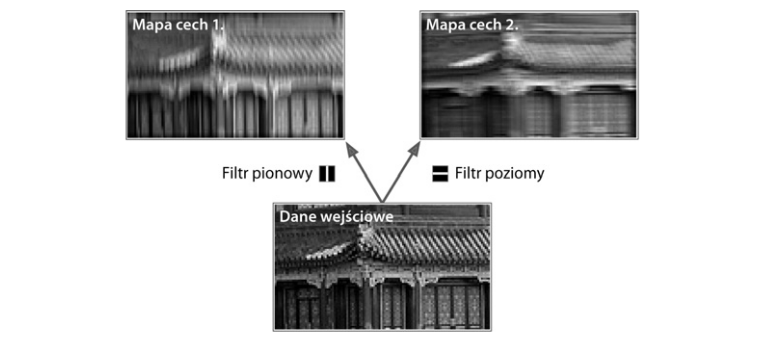
\includegraphics[width=0.9\linewidth]{rys/cnn_filtry.png}
	\caption{Uzyskiwanie dwóch map cech za pomocą dwóch różnych filtrów}
	\zrodlo{\cite{geron}}
	\label{fig:filtry}
\end{figure}

\begin{uwaga}[Wielkość jądra]
	Jądro (zwane również filtrem lub polem receptywnym) typowo ma wysokość i szerokość trzech pikseli. Rozmiar ten okazał się optymalny w szerokim zakresie zastosowań widzenia maszynowego w nowoczesnych sieciach konwolucyjnych. Popularna jest również wielkość 5x5 pikseli, a maksymalny stosowany rozmiar to 7x7 pikseli. Jeśli jądro jest zbyt duże w stosunku do obrazu, wtedy w polu receptywnym pojawia się zbyt wiele cech i warstwa konwolucyjna nie jest w stanie się skutecznie uczyć. Jeżeli jądro jest zbyt małe, np. ma wymiary 2x2 piksele, nie jest w stanie dopasować się do żadnej struktury, przez co jest bezużyteczne \cite{illustrated}.
\end{uwaga}

\subsubsection{Stosy map cech}

Do tej pory dla uproszczenia przedstawialiśmy każdą warstwę splotową w postaci cienkiej, dwuwymiarowej warstwy, ale w rzeczywistości składa się ona z kilku map cech o identycznych rozmiarach, dlatego trójwymiarowe odwzorowanie jest bliższe rzeczywistości (rysunek \ref{fig:warstwy-kanaly}). W zakresie jednej mapy cech każdy neuron jest przydzielony do jednego piksela, a wszystkie tworzące ją neurony współdzielą te same parametry (wagi i człon obciążenia). Neurony w innych mapach cech mają odmienne wartości parametrów. Pole recepcyjne neuronu nie ulega zmianie, ale „przebiega” przez
wszystkie mapy cech poprzednich warstw. Krótko mówiąc, warstwa splotowa równocześnie stosuje
różne filtry na wejściach, dzięki czemu jest w stanie wykrywać wiele cech w dowolnym obszarze obrazu.

\begin{figure}[!h]
	\centering
	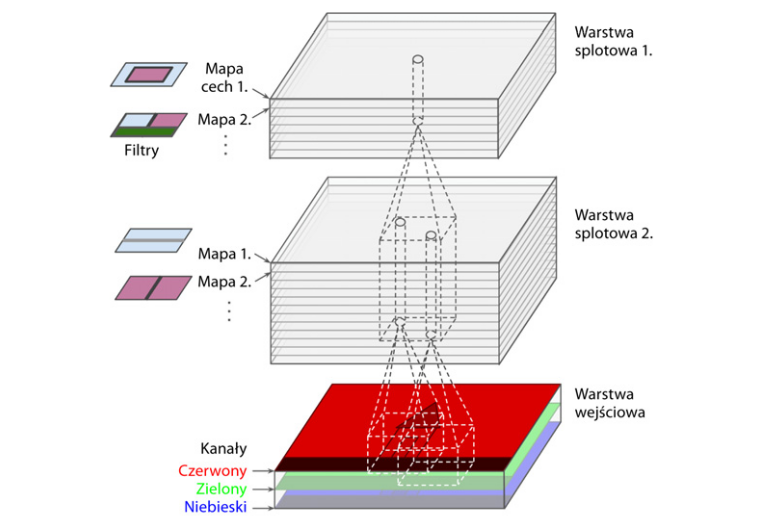
\includegraphics[width=\linewidth]{rys/warstwy_cnn_kanaly.png}
	\caption{Warstwy splotowe zawierające wiele map cech, a także zdjęcie z trzema kanałami barw}
	\zrodlo{\cite{geron}}
	\label{fig:warstwy-kanaly}
\end{figure}

Co więcej, obrazy wejściowe także składają się z kilku warstw podrzędnych, po jednej na każdy \textbf{kanał
barw} (ang. \emph{color channel}). Standardowo występują trzy kanały barw — czerwony, zielony i niebieski
(ang. red, green, blue — RGB). Obrazy czarno-białe (w odcieniach szarości) zawierają tylko jeden
kanał, ale istnieją też takie zdjęcia, które mogą mieć ich znacznie więcej — np. fotografie satelitarne
utrwalające dodatkowe częstotliwości fal elektromagnetycznych (takie jak podczerwień).

W szczególności neuron zlokalizowany w rzędzie $i$ oraz kolumnie $j$ mapy cech $k$ w danej warstwie
splotowej $l$ jest połączony z neuronami wcześniejszej warstwy $l-1$ umieszczonymi w rzędach od $i\times s_h$
do $i\times s_h +f_h -1$ i kolumnach od $j\times s$ w do $j\times s_w +f_w -1$ we wszystkich mapach cech (warstwy $l-1$). Wszystkie neurony znajdujące się w tym samym rzędzie $i$ oraz kolumnie $j$, ale w innych
mapach cech są połączone z wyjściami dokładnie tych samych neuronów poprzedniej warstwy.



Powyższy opis został podsumowany następującym wzorem, służącym do obliczania wyniku danego neuronu w warstwie splotowej:
$$z_{i,j,k}=b_k\sum_{u=0}^{f_h-1}\sum_{v=0}^{f_w-1}\sum_{k'=0}^{f_{n'}-1}x_{i', j', k'} \cdot w_{u,v,k', k},\text{~~~gdzie }\begin{cases}
i'=i \times s_h+u\\
j'=j \times s_w+v
\end{cases}$$
W tym równaniu:
\begin{itemize}
	\item $z_{i,j,k}$ jest wyjściem neuronu znajdującego się w rzędzie $i$, kolumnie $j$ i mapie cech $k$ warstwy
	splotowej $l$;
	\item jak już zostało wyjaśnione, $s_h$ i $s_w$ to kroki pionowy i poziomy, $f_h$ i $f_w$ są wysokością i szerokością
	pola recepcyjnego, natomiast $f_{n'}$ oznacza liczbę map cech w poprzedniej warstwie $(l-1)$;
	\item $x_{i',j',k'}$ jest wyjściem neuronu zlokalizowanego w warstwie $l-1$, rzędzie $i'$, kolumnie $j'$, mapie
	cech $k$ (lub kanale $k'$, jeżeli poprzednia warstwa była warstwą wejściową);
	\item $b_k$ to człon obciążenia dla mapy cech $k$ (w warstwie $l$); można go interpretować jako „pokrętło
	jasności” mapy cech $k$;
	\item $w_{u,v,k',k}$ jest wagą połączenia pomiędzy dowolnym neuronem w mapie cech $k$ warstwy $l$ a jego
	wejściem mieszczącym się w wierszu $u$, kolumnie $v$ (względem pola recepcyjnego neuronu)
	a mapą cech $k'$.
\end{itemize}



\subsubsection{Warstwa łącząca}

Przejdźmy teraz do drugiego elementu budulcowego sieci CNN — \textbf{warstwy łączącej}, zwanej czasem redukującą (ang. pooling layer). Warstwa konwolucyjna może zawierać dowolną liczbę jąder, z których każde generuje mapę aktywacji. Zatem wyjście warstwy konwolucyjnej jest trójwymiarowa tablica aktywacji, której głębokość jest równa liczbie filtrów. Warstwa redukująca zmniejsza przestrzenny wymiar mapy aktywacji, pozostawiając jej głębokość bez zmian \cite{illustrated}. Jej celem jest podpróbkowanie
(ang. subsample; tj. zmniejszenie) obrazu wejściowego w celu zredukowania obciążenia obliczeniowego,
wykorzystania pamięci i liczby parametrów (a tym samym ograniczenia ryzyka przetrenowania).
Podobnie jak w przypadku warstw splotowych, każdy neuron stanowiący część warstwy łączącej
łączy się z wyjściami określonej liczby neuronów warstwy poprzedniej, mieszczącej się w obszarze
niewielkiego, prostokątnego pola recepcyjnego. Podobnie jak wcześniej, musimy definiować tu
rozmiar tego pola, wartość kroku, rodzaj uzupełniania zerami itd. Jednakże warstwa łącząca nie zawiera
żadnych wag; jej jedynym zadaniem jest gromadzenie danych wejściowych za pomocą jakiejś funkcji agregacyjnej, np. maksymalizującej lub uśredniającej. Na rysunku \ref{fig:max-pooling-layer} widzimy najpopularniejszy
rodzaj — \textbf{maksymalizującą warstwę łączącą} (ang. max pooling layer). W tym przykładzie korzystamy
z \textbf{jądra łączącego}  (ang. pooling kernel) o rozmiarze 2×2, kroku o wartości 2 i z pominięciem uzupełniania zerami. Jedynie maksymalna wartość z każdego jądra zostaje przekazana do następnej warstwy natomiast pozostałe wartości wejściowe zostają odrzucone. Na przykład w lewym dolnym polu recepcyjnym na rysunku \ref{fig:max-pooling-layer} widzimy wartości wejściowe 1, 5, 3, 2, zatem tylko wartość maksymalna, czyli 5, zostanie przekazana do następnej warstwy. Z powodu kroku równego 2 obraz wyjściowy ma szerokość i wysokość o połowę mniejsze w porównaniu do obrazu wejściowego (zaokrąglamy tu w dół, ponieważ nie korzystamy z uzupełniania zerami).

\begin{figure}[!h]
	\centering
	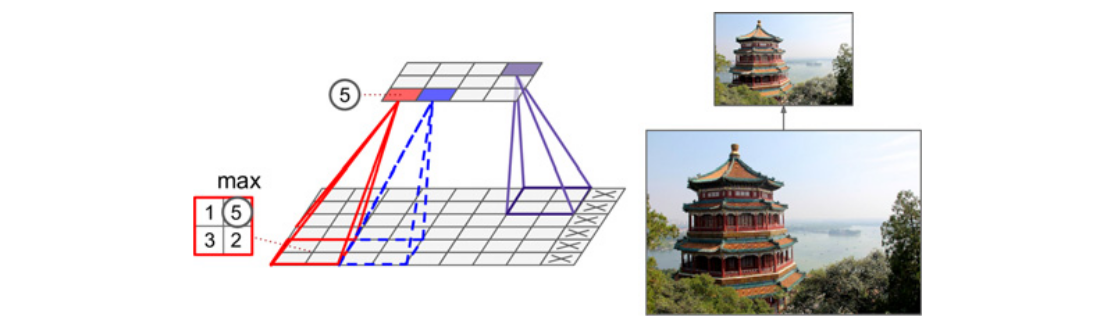
\includegraphics[width=\linewidth]{rys/max_pooling_layer.png}
	\caption{Maksymalizująca warstwa łącząca (jądro łączące: 2×2, krok: 2, brak uzupełniania zerami)}
	\zrodlo{\cite{geron}}
	\label{fig:max-pooling-layer}
\end{figure}

\begin{uwaga}[Parametry warstwy redukującej]
	 Filtr w warstwie redukującej ma zazwyczaj wymiary 2x2 piksele, a krok ma długość dwóch pikseli. W takim wypadku filtr w każdej pozycji przetwarza cztery wartości aktywacji, wybiera największą i w efekcie czterokrotnie redukuje liczbę aktywacji \cite{illustrated}.
\end{uwaga}

\newpage

Na rysunku \ref{fig:max-polling} widoczne jest działanie maksymalizującej warstwy redukującej na mapie aktywacji o wymiarze 4x4. Filtr przesuwa się nad danymi wejściowymi od lewej do prawej, od góry do dołu, tak jak w warstwie konwolucyjnej, i w każdej zajmowanej pozycji przeprowadza operację redukcji danych. W tym przykładzie filtr i krok mają rozmiar 2x2. Skutkuje to otrzymaniem mapy cztery razy mniejszej niż oryginalna.

\begin{figure}[!h]
	\centering
	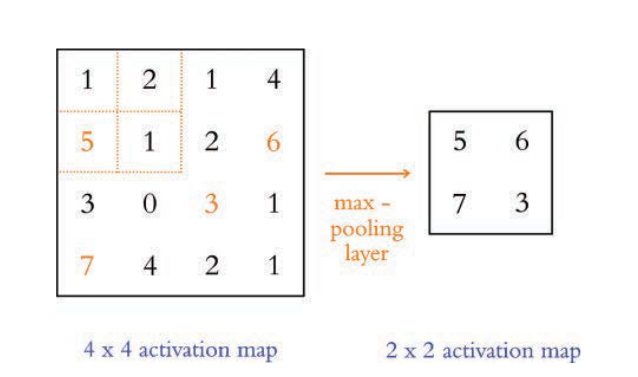
\includegraphics[width=\linewidth]{rys/max-polling.png}
	\caption{Warstwa \emph{max-pooling} z filtrem i krokiem rozmiaru 2x2, zastosowana do mapy aktywacji o rozmiarze 4x4 (widoczna po lewej stronie) skutkuje uzyskaniem mapy czterokrotnie mniejszej niż oryginalna}
	\zrodlo{\cite{illustrated}}
	\label{fig:max-polling}
\end{figure}

Oprócz ograniczania liczby obliczeń, zużycia pamięci i liczby parametrów maksymalizująca warstwa łącząca wprowadza także pewien stopień \textbf{niezmienniczości} w stosunku do drobnych przesunięć, co widać na rysunku \ref{fig:niezmienniczosc-pooling}. Zakładamy tu, że piksele jasne mają mniejszą wartość od pikseli
ciemnych, trzy obrazy (A, B i C) przechodzą przez maksymalizującą warstwę łączącą o jądrze 2×2
i kroku równym 2. Obrazy B i C wyglądają tak samo jak obraz A, ale są przesunięte o, odpowiednio, jeden i dwa piksele w prawo. Jak widać, rezultaty wygenerowane w maksymalizującej warstwie łączącej z obrazów A i B są identyczne. Na tym polega \textbf{niezmienniczość przesunięć} (ang. translation invariance). W przypadku obrazu C wynik jest odmienny: jest on przesunięty o jeden piksel w prawo (nadal jednak pozostaje niezmieniony w mniej więcej 75\%). Poprzez wstawianie maksymalizującej warstwy łączącej co kilka warstw sieci CNN możliwe jest uzyskanie ograniczonej niezmienniczości przesunięć w większej skali. Ponadto warstwa ta zapewnia niewielki stopień niezmienniczości rotacyjnej i drobną niezmienniczość skalowania. Tego typu niezmienniczość (mimo że jest ograniczona) przydaje się wszędzie tam, gdzie prognozy nie powinny być zależne od tych szczegółów, na przykład w zadaniach klasyfikacji.

\begin{figure}[!h]
	\centering
	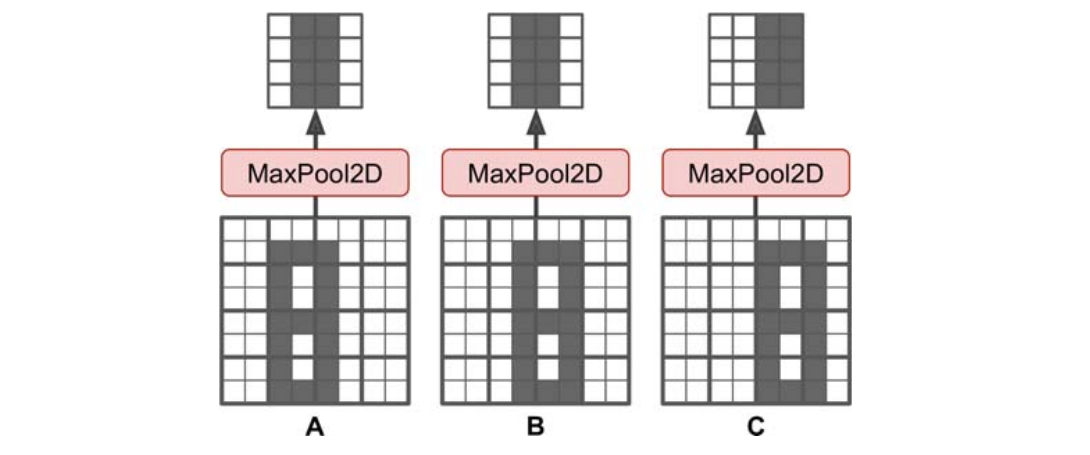
\includegraphics[width=\linewidth]{rys/niezmienniczosc_pooling.png}
	\caption{Niezmienniczość związana z drobnymi przesunięciami}
	\zrodlo{\cite{geron}}
	\label{fig:niezmienniczosc-pooling}
\end{figure}



Jednak maksymalizująca warstwa łącząca jest niepozbawiona również wad. Przede wszystkim jest
ona bardzo niszczycielska: nawet w przypadku niewielkiego jądra o rozmiarze 2×2 i kroku o wartości 2
dane wyjściowe będą dwukrotnie mniejsze w każdym kierunku (zatem obszar obrazu będzie
zmniejszony czterokrotnie), co oznacza porzucenie 75\% wartości wejściowych. Z kolei w pewnych
zastosowaniach niezmienniczość jest niepożądana, na przykład w segmentacji semantycznej (zadaniu
klasyfikowania każdego piksela obrazu zgodnie z jego przynależnością do danego obiektu): jest oczywiste, że jeżeli obraz wejściowy zostanie przesunięty o jeden piksel w prawo, to wynik również powinien być przesunięty w taki sam sposób. Wówczas celem staje się \textbf{ekwiwariancja} (ang. equivariance), a nie niezmienniczość: mała zmiana w sygnale wejściowym
powinna prowadzić do powiązanej z nią niewielkiej zmiany w sygnale wyjściowym.

Podobnie do maksymalizującej warstwy łączącej jest zdefiniowana \textbf{uśredniająca warstwa łącząca} (average pooling layer), która zamiast maksimum używa średniej. Jest ona rzadziej wybierana w zastosowaniach niż warstwa maksymalizująca, z powodu słabszej wydajności. Obliczanie średniej zazwyczaj powoduje mniejszą utratę informacji niż obliczanie maksimum, ale za to warstwa maksymalizująca zachowuje wyłącznie najistotniejsze cechy i ignoruje te mniej ważne, dlatego kolejne warstwy otrzymują coraz czystszy sygnał.

Ostatnim rodzajem warstwy łączącej często spotykanym we współczesnych architekturach jest
\textbf{globalna uśredniająca warstwa łącząca} (ang. global average pooling layer). Mechanizm jej działania
jest całkiem odmienny: oblicza ona jedynie średnią każdej mapy cech (przypomina to działanie
uśredniającej warstwy łączącej, w której jądro ma takie same wymiary przestrzenne jak dane
wejściowe). Oznacza to, że generuje ona na wyjściu pojedynczą wartość na każdą mapę cech
i na każdy przykład. Jest to oczywiście rozwiązanie skrajnie destrukcyjne (większość informacji
zawartych w mapie cech zostaje utraconych), ale, jak przekonasz się w dalszej części rozdziału,
bywa przydatne na wyjściu modelu.


	
\section{Autoenkodery}
	
\subsection{Czym jest autoenkoder}

	\textbf{Autoenkoder} (czasem także nazywany autokoderem, z ang. \textit{autoencoder}, \textit{auto-encoder}) jest rodzajem sieci neuronowej przeznaczonym głównie do kodowania danych wejściowych do skompresowanej i znaczącej reprezentacji, a następnie dekodowania ich z powrotem w taki sposób, aby zrekonstruowane dane były jak najbardziej podobne do oryginalnych \cite{bank}. Autoenkodery uczą się gęstych reprezentacji danych, tzw. \textbf{reprezentacji ukrytych} (ang. \emph{latent representations}) lub \textbf{kodowań} (ang. \emph{codings}) bez jakiejkolwiek formy nadzorowania (tzn. zbiór danych nie zawiera etykiet). Wyjściowe kodowania zazwyczaj mają mniejszą wymiarowość od danych wejściowych, dzięki czemu autoenkodery mogą z powodzeniem służyć do \textbf{redukcji wymiarowości}. Mają też zastosowanie w \textbf{modelach generatywnych} (ang. \emph{generative models}), które potrafią losowo generować nowe dane przypominające zbiór uczący, choć warto zaznaczyć, że często lepszej jakości dane można uzyskać przy użyciu generatywnych sieci przeciwstawnych, czyli GAN (ang. \textit{Generative Adversial Networks}).  \cite{geron}. Autoenkoder jest zatem siecią neuronową szkoloną po to, aby kopiować dane wejściowe do wyjścia. Zawiera ukrytą warstwę $h$, która opisuje kodowanie używane do reprezentowania wejścia. Sieć można postrzegać jako składającą się z dwóch części: kodującej funkcji $h(x)$ i dekodera, który tworzy rekonstrukcję $r=g(h)$  \cite{goodfellow}. Ogólna struktura autoenkodera jest przedstawiona na rysunku \ref{fig:autoencoder_structue}.

\begin{figure}[!h]
	\centering
	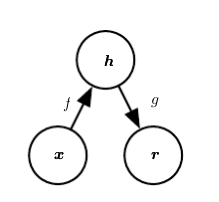
\includegraphics[width=6cm]{rys/autoencoder_structure.png}
	\caption{
		Struktura autoenkoera odwzorowującego wejście $x$ na wyjście $r$ (nazywane rekonstrukcją) poprzez reprezentację ukrytą (kodowanie) $h$. Autoenkoder składa się z dwóch składników: kodera $f$ (odwzorowującego $x$ na $h$) i dekodera $g$ (odwzorowującego $h$ na $r$)}
	\zrodlo{\cite{goodfellow}}
	\label{fig:autoencoder_structue}
\end{figure}

Gdyby autoenkoder nauczył się po prostu, aby na wyjściu ustawiać zawsze $g(f(x))=x$, to nie byłby zbyt przydatny. Z tego powodu autoenkodery są projektowane tak, aby nie potrafiły kopiować w sposób doskonały. Zazwyczaj nakładane są ograniczenia, aby autoenkoder mógł kopiować jedynie w przybliżeniu, i tylko takie dane, które są podobne do danych ze zbioru uczącego. Dzięki temu model musi wybierać jedynie pewne aspekty danych wejściowych, które powinny być kopiowane. W ten sposób może on zdobyć użyteczne informacje o strukturze danych.



%We współczesnych zastosowaniach oprócz deterministycznych funkcji do stochastycznego odwzorowania $p_{encoder}(h|x)$ i $p_{decoder}(x|h)$ stosuje się uogólnioną koncepcję kodera i dekodera.

%Tradycyjnie autoenkodery były używane do redukcji wymiarów lub poznawania cech. Ostatnio teoretyczne powiązania z modelami zmiennych utajonych sprawiły, że autoenkodery znalazły się na pierwszym planie w modelowaniu generatywnym.

Autoenkodery można wyobrazić sobie jako specjalny przypadek sieci jednokierunkowych i można je szkolić, używając wszystkich tych samych technik, zwykle minipakietowego spadku gradientu po gradientach obliczonych przez propagację wstecz. W przeciwieństwie to ogólnych sieci jednokierunkowych, autoenkodery można szkolić za pomocą recyrkulacji, czyli algorytmu uczącego się na bazie porównywania aktywacji sieci na oryginalnym wejściu z aktywacjami na zrekonstruowanym wejściu \cite{goodfellow}. 

\subsection{Rodzaje autoenkoderów}

Jak wspomniano wcześniej, aby autoenkoder był użyteczny, zamiast jedynie kopiować wejście do wyjścia, można na niego nałożyć różne ograniczenia, jak na przykład limit na rozmiar reprezentacji ukrytej. Ze względu na nakładane ograniczenia, wyróżniamy wiele rodzajów autoenkoderów, a wśród nich:
\begin{itemize}
	\item  autoenkodery niedopełnione (ang. \emph{undercomplete}), w których wyjście musi mieć mniejszy wymiar niż wejście
 \item autoenkodery z regularyzacją (ang. \emph{regularized}), w których wyjście ma taki sam lub większy (ang. \emph{overcomplete}) wymiar niż wyjście, ale używają specjalnie dopasowanych funkcji straty. Wśród autoenkoderów z regularyzacją można rozróżnić na przykład:
 \begin{itemize}
 	\item autoenkodery rzadkie (ang. \emph{sparse}), które dążą do rzadkiej reprezentacji ukrytej
 	\item autoenkodery odszumiające (ang. \emph{denoising}), które na wejściu dostają zniekształcone dane, a starają się odzyskać pierwotne, niezaszumione informacje
 	\item autoenkodery kurczliwe (ang. \emph{contractive}) dążące do małego rozmiaru pochodnej
 \end{itemize}
\item autoenkodery stosowe (ang. \emph{stacked}) nazywane również głębokimi (ang. \emph{deep})
\item autoenkodery splotowe (ang. \emph{convolutional})
\item autoenkodery rekurencyjne (ang. \emph{recurrent})
\item autoenkodery wariancyjne (ang. \emph{variational})
\item autoenkodery przeciwstawne (ang. \emph{adversial})
\item autoenkodery stochastyczne (ang. \emph{stochastic})
\end{itemize}
W następnych podrozdziałach zostaną przybliżone cechy charakterystyczne tych rodzajów autoenkoderów.

\subsubsection{Autoenkodery niedopełnione}

Kopiowanie wejścia do wyjścia może wydawać się bezużyteczne, ale wyjście dekodera nas nie interesuje. Mamy za to nadzieję, że skutkiem przeszkolenia autoenkodera do kopiowania będzie kod $h$, mający przydatne właściwości.
Jednym ze sposobów, aby uzyskać przydatne cechy z autoenkodera, jest ograniczenie $h$ do mniejszego wymiaru niż $x$. Autoenkoder, w którym wymiar kodu jest mniejszy niż wymiar wejściowy, jest nazywany niekompletnym (niedopełnionym).
Poznawanie niekompletnych reprezentacji zmusza autoenkoder do przechwycenia najistotniejszych cech danych szkoleniowych.
Proces poznawania jest opisywany po prostu jako minimalizowanie funkcji straty
$$L(x, g(f(x)))$$
gdzie $L$ jest funkcją straty karzącą $g(f(x))$ za niepodobieństwo do $x$ jak np. błąd średniokwadratowy.

Gdy dekoder jest liniowy, a $L$ to błąd średniokwadratowy, niekompletny autoenkoder uczy się obejmować tą samą podprzestrzeń co PCA. W tym przypadku poznanie zasadniczej podprzestrzeni danych szkoleniowych przez szkolony do kopiowania autoenkoder jest efektem ubocznym. Autoenkodery z nieliniowymi funkcjami kodowania $f$ i nieliniowymi funkcjami dekodowania $g$ mogą więc poznawać potężniejsze, nieliniowe uogólnienie PCA. Niestety, jeśli koder i dekoder będą mieć zbyt dużą pojemność, autoenkoder może nauczyć się wykonywać kopiowanie bez wyodrębniania pożytecznych informacji o rozkładzie danych. Teoretycznie można sobie wyobrazić, ze autoenkoder z jednowymiarowym kodem, ale bardzo potężnym nieliniowym koderem, może nauczyć się reprezentować każdy przykład szkoleniowy $x^{(i)}$ za pomocą kodu $i$. Dekoder mógłby nauczyć się odwzorowywać te całkowitoliczbowe indeksy z powrotem na wartości konkretnych przykładów szkoleniowych. Ten konkretny przykład nie występuje w praktyce, ale pokazuje wyraźnie, że autoenkoder przeszkolony do wykonywania kopiowania może zawieść, jeśli chodzi o poznanie czegoś przydatnego na temat zbioru danych, jeśli pozwoli się, aby miał za dużą pojemność \cite{goodfellow}.

\subsubsection{Autoenkodery z regularyzacją}



W przypadku, gdy wymiar wyjścia jest większy (autoenkodery nadkompletne) lub równy niż wymiar wejścia, nawet liniowy koder i dekoder mogą nauczyć się kopiować wejście do wyjścia bez uczenia się niczego przydatnego na temat rozkładu danych.

Ideałem byłaby możliwość udanego szkolenia dowolnej architektury autoenkodera przy wyborze wymiaru kodu oraz pojemności kodera i dekodera na podstawie złożoności rozkładu modelowanego. Można to zrobić, stosując regularyzację. Zamiast ograniczać pojemność modelu przez zachowywanie płytkości kodera i dekodera oraz małego rozmiaru kodu, autoenkodery z regularyzacją używają funkcji straty, dzięki której model może posiadać inne właściwości oprócz możliwości kopiowania swojego wejścia do wyjścia. Do tych właściwości należą:

\begin{itemize}
	\item  rzadkość reprezentacji
	\item mały rozmiar pochodnej reprezentacji
	\item odporność na szum lub brakujące dane wejściowe
\end{itemize}

Autoenkoder z regularyzacją może być nieliniowy i nadkompletny, a mimo to nauczyć się czegoś wartościowego o rozkładzie danych, nawet jeśli pojemność modelu jest na tyle duża, aby poznać trywialną funkcję tożsamościową \cite{goodfellow}.

\subsubsection{Rzadkie autoenkodery}

Rzadkie autoenkodery są zwykle używane do tego, aby uczyć się cech do innego zadania, takiego jak klasyfikacja. Autoenkoder, który dzięki regularyzacji jest rzadki, musi reagować na unikatowe statystyczne cechy zbioru danych, na którym został wyszkolony, a nie tylko działać jak funkcja tożsamościowa.

Kryterium szkolenia autoenkodera rzadkiego obejmuje karę rzadkości $\Omega(h)$ na warstwie kodu $h$ oprócz błędu rekonstrukcji
$$L(x, g(f(x)))+\Omega(h)$$
gdzie $g(h)$ to wyjście dekodera, a zwykle mamy $h=f(x)$, czyli wyjście kodera \cite{goodfellow}. Dodanie tego składnika do funkcji kosztu zmusza autoenkoder do zmniejszenia liczby aktywnych neuronów w warstwie kodowania. W ten sposób każde wejście musi być reprezentowane jako kombinacja niewielkiej iczby pobudzeń. Dzięki temu każdy neuron warstwy kodowania zazwyczaj uczy się wykrywać jakąś przydatną cechę \cite{geron}.

W każdym przebiegu uczenia następuje pomiar rzeczywistej rzadkości warstwy kodowania i karanie modelu, gdy zmierzona rzadkość różni się od docelowej. W tym celu obliczania jest średnia aktywacja każdego neuronu w warstwie dla całej grupy przykładów uczących. Rozmiar tej grupy nie może być zbyt mały, aby wyliczona wartość średniej była dokładna. Następnie nakładana jest kara na zbyt aktywne neurony, poprzez dodanie funkcji straty rzadkości (ang. \emph{sparsity loss}) $\Omega(h)$ do funkcji kosztu. Dla przykładu, jeśli średnia wartość aktywacji neuronu to 0.3, ale docelowo powinna wynosić 0.1, musimy ją zmniejszyć. Jednym ze sposobów jest dodanie kwadratu błędu $(0.3-0.1)^2$ do funkcji kosztu. Lepszym rozwiązaniem w praktyce jest zastosowanie dywergencji Kullbacka-Leiblera, której gradienty są znacznie większe niż w błędzie średniokwadratowym (rysunek \ref{fig:funkcja-straty-rzadkosci}).



\begin{figure}[!h]
	\centering
	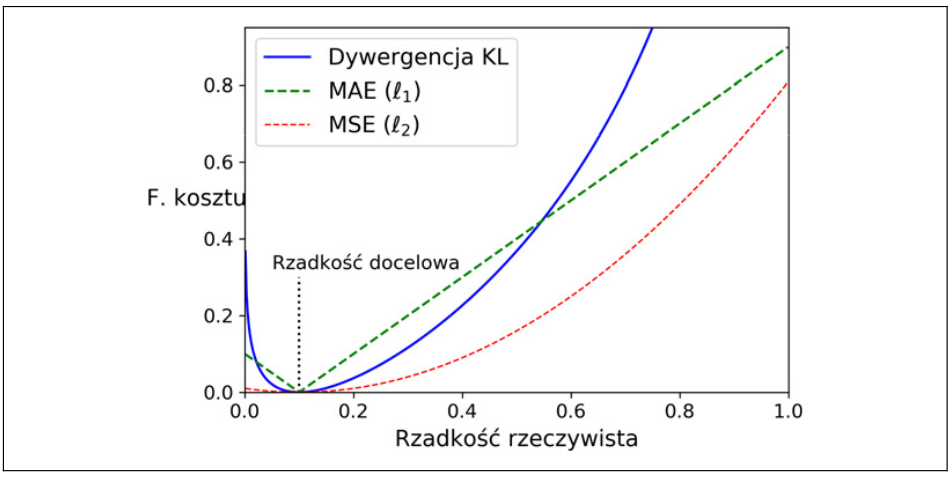
\includegraphics[width=\linewidth]{rys/funkcja_straty_rzadkosci.png}
	\caption{Funkcje straty rzadkości}
	\zrodlo{\cite{geron}}
	\label{fig:funkcja-straty-rzadkosci}
\end{figure}

Mając dwa dyskretne rozkłady prawdopodobieństwa P i Q, możemy obliczyć rozbieżność pomiędzy nimi $D_{KL}(P||Q)$ za pomocą dywergencji Kullbacka-Leiblera:
$$D_{KL}(P||Q)=\sum_i P(i)\log \frac{P(i)}{Q(i)}$$

W przypadku autoenkodera rzadkiego naszym celem jest zmierzenie rozbieżności pomiędzy docelowym prawdopodobieństwem $p$ aktywacji neuronu w warstwie kodowania, a rzeczywistym prawdopodobieństwem $q$ (które jest średnią aktywacją dla danych uczących). Dywergencję KL można wówczas zapisać jako:
$$D_{KL}(p||q)=p\log \frac{p}{q}+(1-p)\log \frac{1-p}{1-q}$$

Po obliczeniu funkcji straty rzadkości dla każdego neuronu w warstwie kodowania, należy je zsumować i wynik dodać do funkcji kosztu. W celu regulowania względnej istotności funkcji straty rzadkości i funkcji straty rekonstrukcji, można tą pierwszą pomnożyć przez hiperparametr wagi rzadkości. Jeśli wartość tego hiperparametru będzie zbyt duża, to model pozostanie blisko rzadkości docelowej, ale jednocześnie nie będzie w stanie prawidłowo rekonstruować danych wejściowych. Przy zbyt małej wartości tego parametru, model będzie ignorował cel rzadkości \cite{geron}.




\subsubsection{Autoenkodery z odszumianiem}
Zamiast dodawać karę $\Omega$ do funkcji kosztów, możemy uzyskać autoenkoder, który uczy się czegoś przydatnego, zmieniając składnik błędu rekonstrukcji w funkcji kosztów. Tradycyjne autoenkodery minimalizują jakąś funkcję
$$L(x, g(f(x)))$$
gdzie $L$ to funkcja straty karząca $g(f(x))$ za niepodobieństwo do $x$, jak np. norma $L^2$ ich różnicy. Sprzyja to temu, aby $g \circ f$  uczyła się być jedynie funkcją tożsamościową, jeśli ma do tego odpowiednią pojemność.

Autoenkoder z odszumianiem zamiast tego minimalizuje
$$L(x, g(f(\tilde{x})))$$
gdzie $\tilde{x}$ to kopia $x$, która została zniekształcona przez jakiegoś rodzaju postać szumu. Autoenkodery mają tym samym za zadanie odwrócić to zniekształcenie, a nie po prostu przekopiować swoje wejście \cite{goodfellow}.

Zniekształcenie może być szumem gaussowskim dodawanym do danych wejściowych lub może przybrać postać losowo wyłączanych wejść za pomocą metody porzucania. Autoenkodery z takimi zniekształceniami zostały przedstawione na rysunku \ref{fig:autoenkoder-odszumiajacy}.


%Implementacja nie stanowi wyzwania: jest to standardowy autokoder stosowy zawierający dodatkową warstwę Dropout , przez którą przechodzą dane wejściowe (możesz zastąpić ją warstwą GaussianNoise ). Jak pamiętamy, warstwa Dropout jest aktywna jedynie w fazie uczenia (podobnie jak warstwa GaussianNoise ):



\begin{figure}[!h]
	\centering
	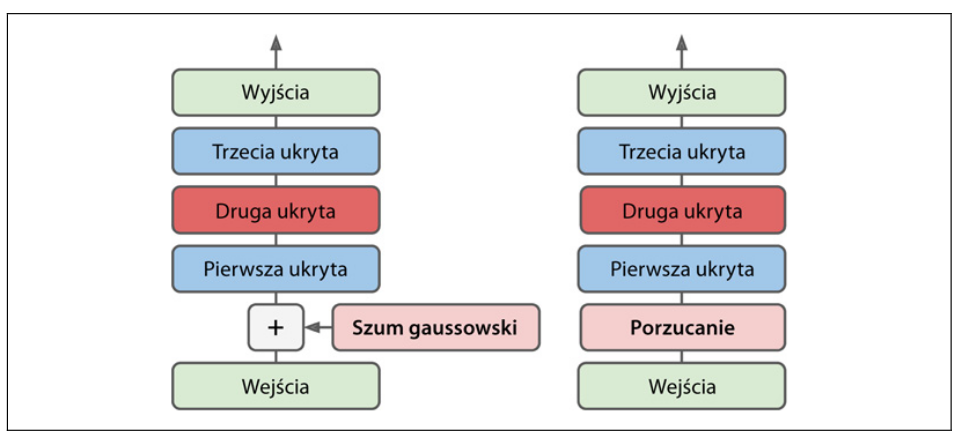
\includegraphics[width=\linewidth]{rys/autoenkoder_odszumiajacy.png}
	\caption{Autokodery odszumiające: wykorzystujące szum gaussowski (po lewej) lub metodę porzucania
		(po prawej)}
	\zrodlo{\cite{geron}}
	\label{fig:autoenkoder-odszumiajacy}
\end{figure}


Rysunek \ref{fig:autoenkoder-denoising} przedstawia przykłady zaszumionych obrazów (połowa pikseli została „wyłączona”), a także ich rekonstrukcje uzyskane za pomocą autokodera odszumiającego (bazującego na warstwie porzucania). Autokoder  „odgaduje” szczegóły niewystępujące w obrazach wejściowych, na przykład górną część białej sukienki (czwarty obraz w dolnym rzędzie). 

\begin{figure}[!h]
	\centering
	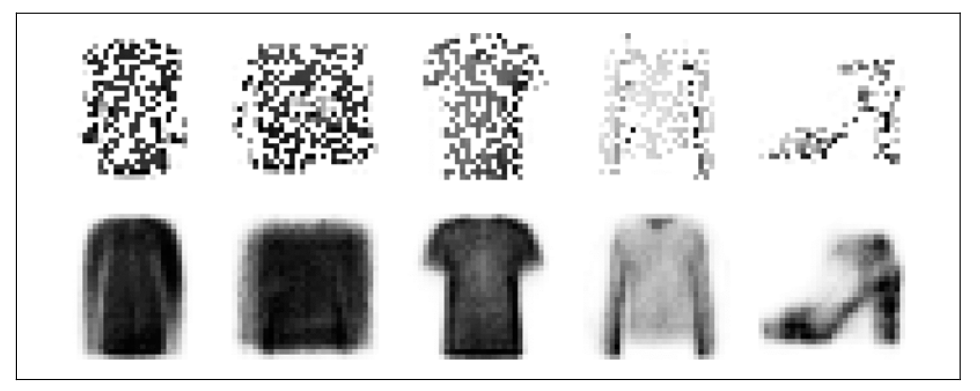
\includegraphics[width=\linewidth]{rys/denoising.png}
	\caption{Zaszumione obrazy (na górze) i ich rekonstrukcje (na dole)}
	\zrodlo{\cite{geron}}
	\label{fig:autoenkoder-denoising}
\end{figure}

Ogólna struktura autoenkodera odszumiającego została przedstawiona na rysunku \ref{fig:denoising-structure}. Wejściem jest zanieczyszczony obraz, a docelową wartością jest oryginał bez zniekształcenia. Sieć uczy się rozpoznawać i usuwać zniekształcenia, aby wygenerować rekonstrukcję. Autoenkoder nnie widzi oryginalnego, czystego obrazu, jedynie ten ze zniekształceniem. 

\begin{figure}[!h]
	\centering
	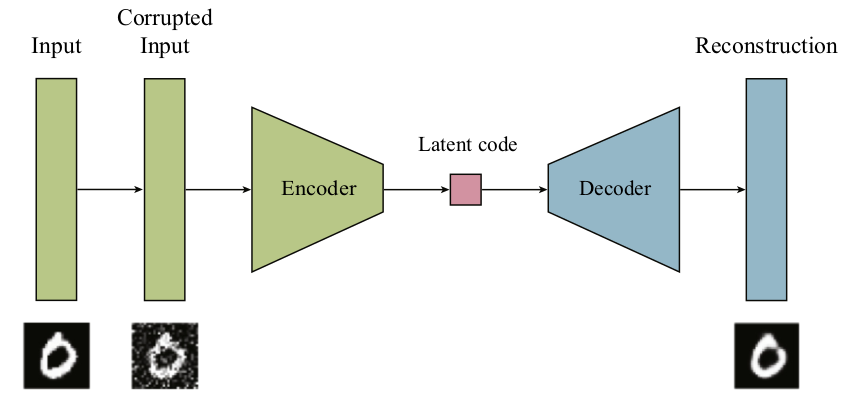
\includegraphics[width=\linewidth]{rys/denoising_autoencoder.png}
	\caption{Struktura autoenkodera odszumiającego}
	\label{fig:denoising-structure}
\end{figure}




\subsubsection{Regularyzacja poprzez karanie pochodnych}

kolejną strategią regularyzacji autoenkodera jest użycie kary $\Omega$ tak, jak w rzadkich autoenkoderach
$$L(x, g(f(x)))+\Omega(h,x)$$
ale z inną postacią $\Omega$:
$$\Omega(h, x)=\lambda \sum_i ||\nabla_x h_i ||^2$$
Zmusza to model do poznania funkcji, która nie zmienia się za bardzo przy niewielkich zmianach $x$. Ponieważ kara ta jest stosowana tylko w przykładach szkoleniowych, zmusza autoenkoder do poznawania cech, które przechwytują informacje o rozkładzie szkoleniowym.

Autoenkoder z taką regularyzacją jest nazywany \textbf{kurczliwym} \cite{goodfellow}.
\subsubsection{Autoenkodery stosowe}


Podobnie jak inne sieci neuronowe, również autoenkodery mogą mieć wiele warstw ukrytych. Takie autoenkodery są nazywane \textbf{stosowymi} (ang. \emph{stacked}) lub \textbf{głębokimi} (ang. \emph{deep}). Dzięki wielu warstwom ukrytym, autoenkoer może się uczyć bardziej skomplikowanych kodowań. Pojawia się jednak niebezpieczeństwo stworzenia modelu zbyt potężnego, podobnie jak zostało to opisane przy autoenkoderach niedopełnionych, gdzie podano teoretyczny przykład autoenkodera przekształcającego $i$-ty przykład uczący na pojedynczą liczbę.

Przykładowa struktura autoenkodera stosowego została przedstawiona na rysunku \ref{fig:autoenkoder-stosowy}. Zazwyczaj architektura autoenkodera stosowego jest symetryczna względem jego centralnej warstwy ukrytej, tak jak widać na rysunku. 
W przypadku symetrycznych autoenkoderów, często stosowane jest \textbf{wiązanie wag} (ang. \emph{tying weights}) warstw kodera z wagami warstw dekodera. W ten sposób liczba wag w modelu zostaje zredukowana o połowę, co przyspiesza proces uczenia i zmniejsza ryzyko przetrenowania modelu. Jeśli autoenkoder zawiera $N$ warstw (oprócz warstwy wejściowej), a $W_L$ oznacza wagi połączeń w $L$-tej warstwie, to wagi warstwy dekodera można zdefiniować jako $W_{N-L+1}=W_L^T$ (dla $L=1,2,\ldots, N/2$).

W celu zaoszczędzenia czasu można zamiast uczyć cały autoenkoder stosowy na raz, trenować pojedyncze składowe osobno, a na koniec połączyć je w całość. To rozwiązanie nazywane jest ,,zachłannym uczeniem warstwowym''. Obecnie jest rzadko stosowane \cite{geron}.

\begin{figure}[!h]
	\centering
	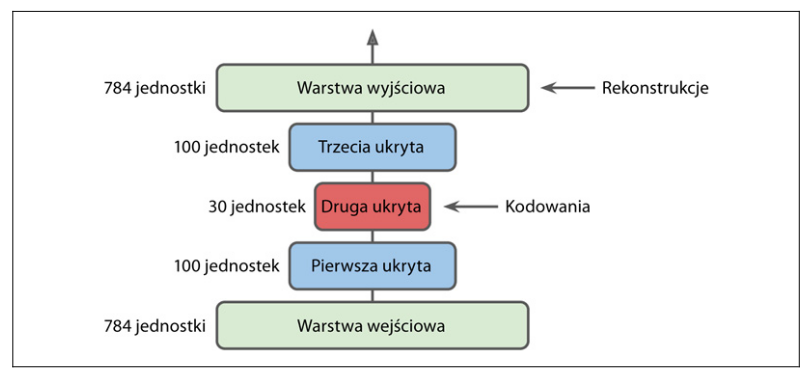
\includegraphics[width=\linewidth]{rys/autoenkoder_stosowy.png}
	\caption{Przykładowa struktura autoenkodera stosowego}
	\zrodlo{\cite{geron}}
	\label{fig:autoenkoder-stosowy}
\end{figure}

\newpage

\subsubsection{Autoenkoder splotowy}

Autoenkodery splotowe są typem autoenkoderów, który najlepiej nadaje się do przetwarzania obrazów. W takim rodzaju autoenkodera, koderem jest sieć konwolucyjna składająca się z warstw splotowych i redukujących. Zwykle zmniejsza ona wymiarowość obrazu (wysokość i szerokość), a zwiększa głębokość (liczbę map cech). Dekoder przeprowadza operację odwrotną: musi zwiększyć rozdzielczość i zredukować głębokość do pierwotnego wymiaru. W tym celu można wykorzystać transponowane warstwy splotowe \cite{geron}.




\subsubsection{Autoenkoder rekurencyjny}

Autoenkodery rekurencyjne zwykle służą do przetwarzania danych sekwencyjnych, takich jak szeregi czasowe czy tekst. W przypadku takiego autoenkodera, koderem zwykle jest sieć sekwencyjno-wektorowa która kompresuje sekwencję wejściową do pojedynczego wektora. Dekoderem jest sieć wektorowo-sekwencyjna odwracająca tą operację \cite{geron}.






\subsubsection{Autoenkoder przeciwstawny}



Ograniczeniem wielu rodzajów auroenkoderów jest to, że nie generują one dobrze ustrukturyzowanej przestrzeni ukrytej. Dzieje się tak dlatego, że podczas uczenia, różne obserwacje ze zbioru zostają zakodowane w sposób losowo rozproszony w przestrzeni ukrytej. W rezultacie rozmieszczenie reprezentacji ukrytych czasami zawiera puste miejsca w przestrzeni ukrytej, co widać na rysunku \ref{fig:latent-spaces}. W tych pustych miejscach znajdują się kodowania $h$, których dekoder nigdy nie uczył się rekonstruować. Dlatego też proces generowania nowych danych z losowo wybranego kodowania $h$ może być trudny. W praktyce rekonstrukcja próbek z tych pustych miejsc zwykle jest błędna. Ogranicza ona zastosowanie niektórych rodzajów autoenkoderów jako modeli generatywnych \cite{pinaya}.


\begin{figure}[!h]
	\centering
	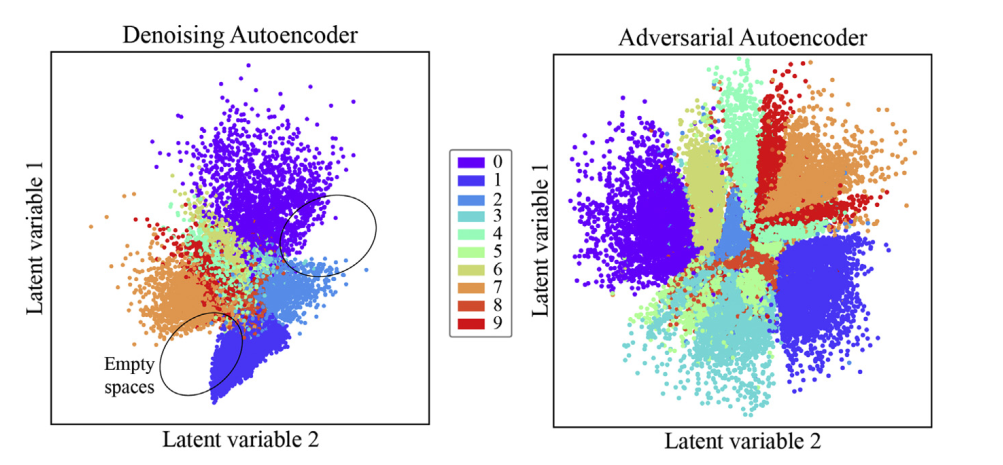
\includegraphics[width=\linewidth]{rys/adversial_autoencoder.png}
	\caption{Reprezentacje ukryte. W tym przykładzie, obrazy cyfr od 0 do 9 były użyte do trenowania autoenkodera odszumiającego i przeciwstawnego. W obu przypadkach dane uczące są przedstawione w dwuwymiarowej przestrzeni ukrytej. Ponieważ nie nakładamy żadnych ograniczeń na autoenkoder odszumiający, to jego przestrzeń ukryta zawiera puste miejsca. Z drugiej strony, autoenkoder przeciwstawny ogranicza reprezentacje do podobnych według rozkładu (w tym przypadku dwuwymiarowego normalnego), co w rezultacie oznacza brak pustych miejsc}
	\zrodlo{\cite{pinaya}}
	\label{fig:latent-spaces}
\end{figure}

Jedną z metod pozwalających na kontrolowanie struktury przestrzeni ukrytej jest stosowanie autoenkodera przeciwstawnego. Ten rodzaj autoenkodera jest połączeniem ogólnego modelu autoenkodera z podejściem trenowania przeciwstawnego, typowego dla generatywnych sieci przeciwstawnych (GAN). Generatywne sieci przeciwstawne składają się z dwóch sieci neuronowych, które konkurują ze sobą, aby polepszyć swoje działanie (rysunek \ref{fig:gan-structure}). Pierwsza sieć to generator, który na wejściu dostaje losowe wartości i stara się wygenerować sztuczne dane, możliwie jak najbardziej podobne do prawdziwych danych. Drugą siecią jest dyskryminator, który decyduje, czy jego wejście pochodzi z generatora czy z prawdziwego zbioru. Celem generatora jest ,,oszukać'' dyskryminator. Obie sieci są trenowane równocześnie, a generator nie ma bezpośredniego dostępu do prawdziwego zbioru danych. Jedynym jego sposobem na poprawę działania jest interakcja z dyskryminatorem. Na podstawie informacji zwrotnych z dyskryminatora, generator stara się dopasować swoją sieć tak, by produkować wyjścia będące dla dyskryminatora trudne do zidentyfikowania jako fałszywe, czyli bardziej podobne do realnych danych.


\begin{figure}[!h]
	\centering
	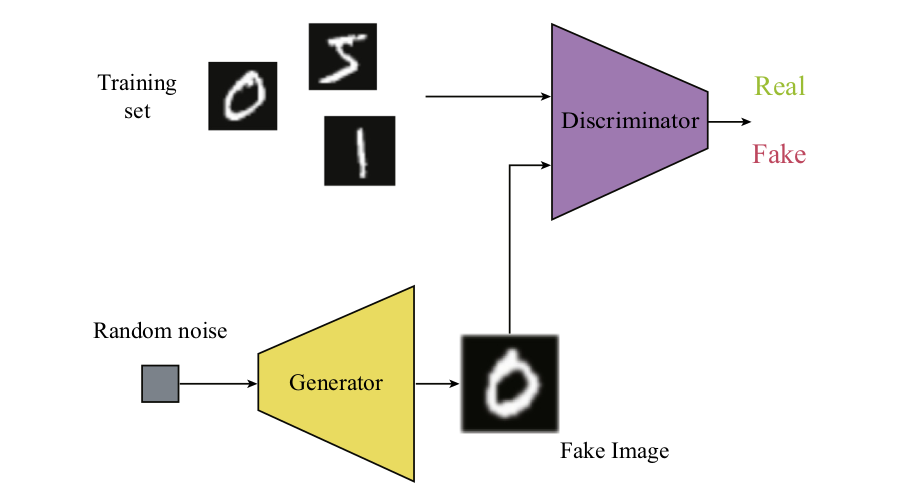
\includegraphics[width=\linewidth]{rys/gan_structure.png}
	\caption{Struktura generatywnej sieci przeciwstawnej (GAN)}
	\zrodlo{\cite{pinaya}}
	\label{fig:gan-structure}
\end{figure}

Autoenkodery przeciwstawne wykorzystują trenowanie przeciwstawne, by ukształtować rozkład danych wejściowych tak, aby był jak najbardziej podobny do predefiniowanego rozkładu. Jest to osiągane poprzez dodanie sieci dyskryminatora do struktury autoenkodera (rysunek \ref{fig:adversial-ae-structure}). W przypadku autoenkoderów przeciwstawnych, dyskryminator otrzymuje dwa rodzaje danych wejściowych: wartości próbkowane z pożądanego rozkładu (przykładowo losowe wartości z rozkładu normalnego) oraz ukryte reprezentacje $h$ obserwacji ze zbioru uczącego. Co ważne, oba muszą mieć takie same wymiary. Pożądany rozkład może być tu traktowany jako rozkład a priori. Podczas procesu uczenia, dyskryminator dokonuje klasyfikacji dotyczącej tego, czy dane pochodzą z rozkładu a priori czy z kodowań ukrytych.

\begin{figure}[!h]
	\centering
	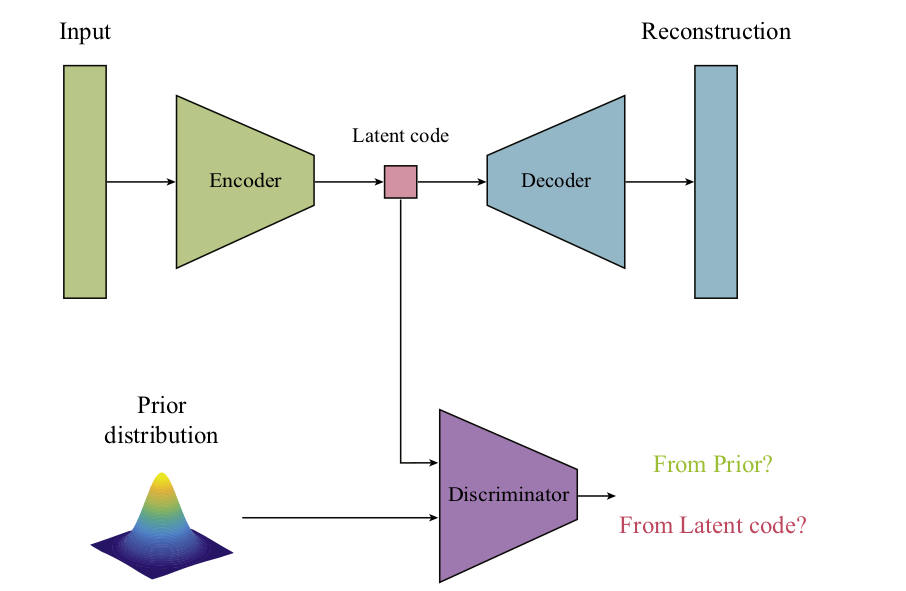
\includegraphics[width=\linewidth]{rys/adversial_ae_structure.png}
	\caption{Struktura autokodera przeciwstawnego. Sieć dyskryminująca jest dodana do autoenkodera, aby zmusić go do generowania reprezentacji ukrytych podobnych do rozkładu a priori}
	\zrodlo{\cite{pinaya}}
	\label{fig:adversial-ae-structure}
\end{figure}

\noindent Gdy w strukturze znajduje się dyskryminator, enkoder jest zmuszony robić jednocześnie dwie rzeczy:

\noindent (i) generować przestrzeń ukrytą, na której może pracować dekoder w celu stworzenia rekonstrukcji wejść

\noindent (ii) generować przestrzeń ukrytą, która oszuka dyskryminator tak, aby klasyfikował kodowania jako próbki z rozkładu a priori

\noindent Innymi słowy, enkoder pełni także rolę generatora.

Trenowanie autoenkodera przeciwstawnego ma trzy kroki w każdej epoce:
 
 \begin{enumerate}

\item Autoenkoder aktualizuje parametry enkodera i dekodera, na podstawie standardowej funkcji straty rekonstrukcji

\item Model aktualizuje parametry sieci dyskryminującej, aby rozróżnić ,,prawdziwe'' próbki (generowane z rozkładu a priori) od wygenerowanych próbek (ukrytych reprezentacji z enkodera)

\item Enkoder na podstawie informacji zwrotnej z dyskryminatora aktualizuje swoje parametry, aby poprawić generowane reprezentacje ukryte, w celu ,,oszukania'' dyskryminatora.

\end{enumerate}

Jeśli proces uczenia się powiedzie, enkoder nauczy się przekształcić rozkład danych wejściowych do rozkładu a priori,  dyskryminator nigdy ni ebędzie pewny, czy dane wejściowe są prawdziwe czy nie, a dekoder uczy się modelu generatywnego, który odwzorowuje narzucony rozkład a priori na rozkład danych wejściowych. Ostatecznie jest możliwe generowanie nowych danych poprzez próbkowanie z rozkładu a priori, przekazanie go do dekodera i pozwolenie mu na wygenerowanie danych.




\subsection{Zastosowania autoenkoderów}




W zadaniach klasyfikacji lub regresji autoenkodery mogą być wykorzystywane do wyodrębniania cech z surowych danych w celu zwiększenia odporności modelu \cite{kumar}. Istnieje wiele innych zastosowań sieci autoenkoderów, które można wykorzystać w różnym kontekście. Omówimy krótko zastosowania takie jak:
\begin{enumerate}
\item  Zmniejszenie wymiarowości (ang. \emph{Dimensionality Reduction })

\item  Wyodrębnianie cech (ang. \emph{Feature Extraction})

\item  Odszumianie obrazu (ang. \emph{Image Denoising })

\item  Kompresja obrazu (ang. \emph{Image Compression})

\item Wyszukiwanie obrazu (ang. \emph{ Image Search })

\item Wykrywanie anomalii (ang. \emph{ Anomaly Detection})

\item  Uzupełnianie brakujących danych (\emph{Missing Value Imputation })

\end{enumerate}

\subsubsection{Zmniejszenie wymiarowości}

(źródło jak wyżej, ale również tu: \url{https://towardsdatascience.com/autoencoders-in-practice-dimensionality-reduction-and-image-denoising-ed9b9201e7e1})

Autoenkodery trenują sieć w celu wyjaśnienia naturalnej struktury danych w efektywnej reprezentacji niskowymiarowej. Osiąga się to poprzez zastosowanie strategii dekodowania i kodowania w celu zminimalizowania błędu rekonstrukcji.

\begin{figure}[!h]
	\centering
	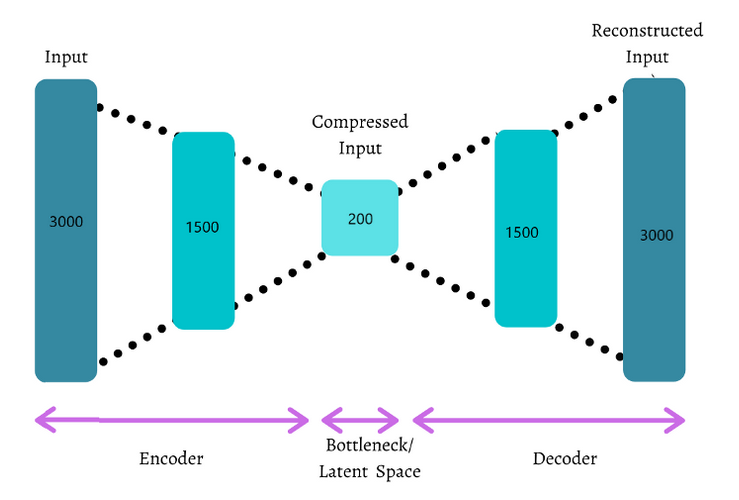
\includegraphics[width=0.8\linewidth]{rys/dimensionality_reduction.png}
	\caption{Redukcja wymiarowości}
	\zrodlo{towards data science}
	\label{fig:dimensionality-reduction}
\end{figure}

Jak widać powyżej, autoenkoder składa się z trzech elementów:

Koder - funkcja służąca do kompresji danych do ich reprezentacji w niższym wymiarze.

Wąskie gardło - nazywane również przestrzenią ukrytą, gdzie nasze początkowe dane są reprezentowane w niższym wymiarze.

Dekoder - funkcja dekompresji lub rekonstrukcji danych o niskim wymiarze z powrotem do wymiaru początkowego.

Wymiar wejściowy i wymiar wyjściowy mają 3000 wymiarów, a pożądany wymiar zredukowany wynosi 200. Możemy stworzyć sieć pięciowarstwową, w której koder ma 3000 i 1500 neuronów, podobnie jak w przypadku sieci dekodera.

Embeddingi wektorowe skompresowanej warstwy wejściowej można traktować jako embedding warstwy wejściowej o zredukowanym wymiarze.


\url{https://towardsdatascience.com/dimensionality-reduction-pca-versus-autoencoders-338fcaf3297d}

Porównanie autokodera niedopełnionego z PCA

- PCA jest liniową transformacją danych, podczas gdy AE mogą być liniowe lub nieliniowe

- PCA jest szybsze niż AE, które używają spadku gradientu 

- PCA gwarantuje ortogonalność wynikowej przestrzeni zmiennych. AE dąży jedynie do jak najmniejszej wartości funkcji straty

- AE są w stanie modelować bardziej złożone lub nieliniowe zależności, podczas gdy PCA jest prostym przekształceniem liniowym

- przy decyzji PCA vs AE, warto wybierać PCA dla mniejszych zbiorów danych, a AE dla większych

- jedynym parametrem metody PCA jest "k" - liczba ortogonalnych wymiarów które chcemy uzyskać. W AE mamy wszystkie hiperparametry architektury sieci neuronowej

- AE z jedną warstwą i liniową funkcją aktywacji ma działanie podobne do PCA. AE z wieloma warstwami i nieliniowymi funkcjami aktywacji (Głębokie AE, Deep AE) są skłonne do przeuczenia, mogą być poprawiane przez regularyzację i odpowiednie zaprojektowanie sieci

\subsubsection{Wyodrębnianie cech}

Autokodery mogą być używane jako ekstraktory cech w zadaniach klasyfikacji lub regresji. Autokodery pobierają nieoznakowane dane i uczą się efektywnych kodowań struktury danych, które mogą być wykorzystane w zadaniach uczenia nadzorowanego.

Po wytrenowaniu sieci auto-enkodera na próbce danych treningowych można zignorować część dekodera auto-enkodera, a jedynie użyć kodera do przekształcenia surowych danych wejściowych o wyższym wymiarze na przestrzeń zakodowaną o niższym wymiarze. Ten niższy wymiar danych może być wykorzystany jako cecha w zadaniach nadzorowanych.

\begin{figure}[!h]
	\centering
	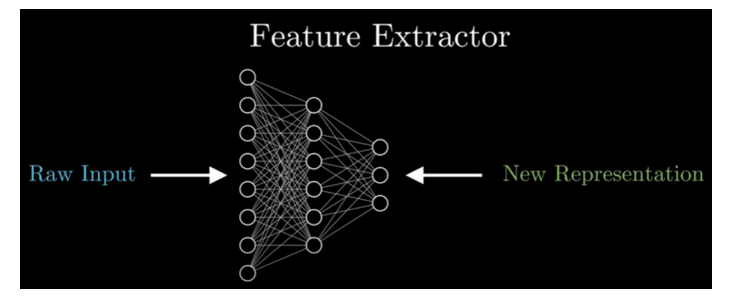
\includegraphics[width=0.8\linewidth]{rys/feature_extractor.png}
	\caption{Wyodrębnianie cech}
	\zrodlo{towards data science}
	\label{fig:feature-extractor}
\end{figure}

\subsubsection{Odszumianie obrazów}

Surowe dane wejściowe ze świata rzeczywistego są często zaszumione, a wytrenowanie solidnego modelu nadzorowanego wymaga danych oczyszczonych i pozbawionych szumu. Do odszumiania danych można wykorzystać autoenkodery.

Jednym z popularnych zastosowań jest odszumianie obrazów, w którym autoenkodery próbują zrekonstruować obraz pozbawiony szumu z zaszumionego obrazu wejściowego.

\begin{figure}[!h]
	\centering
	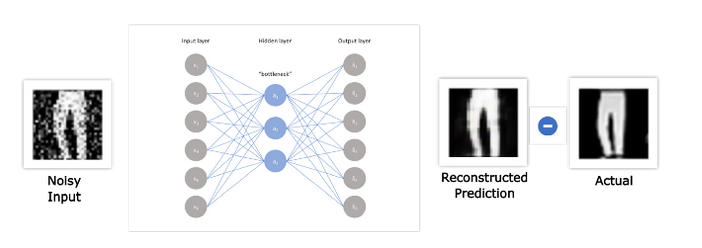
\includegraphics[width=\linewidth]{rys/image_denoising.png}
	\caption{Odszumianie obrazów}
	\zrodlo{towards data science}
	\label{fig:image-denoising}
\end{figure}

Zakłócony obraz wejściowy jest podawany do autoenkodera jako wejście, a bezszumowe wyjście jest rekonstruowane przez minimalizację straty rekonstrukcji w stosunku do oryginalnego wyjścia docelowego (bezszumowego). Po wytrenowaniu wag autoenkodera można je dalej wykorzystać do odszumiania obrazu surowego.

\subsubsection{Kompresja obrazu}

Innym zastosowaniem sieci auto-enkoderów jest kompresja obrazów. Surowy obraz wejściowy można przekazać do sieci kodera i uzyskać skompresowany wymiar zakodowanych danych. Wagi sieci autoenkodera mogą być uczone przez rekonstrukcję obrazu ze skompresowanego kodowania za pomocą sieci dekodera.

\begin{figure}[!h]
	\centering
	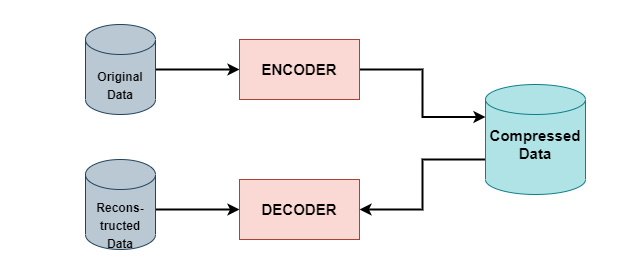
\includegraphics[width=0.8\linewidth]{rys/image_compression.png}
	\caption{kompresja obrazów}
	\zrodlo{towards data science}
	\label{fig:image-compression}
\end{figure}

Zazwyczaj autoenkodery nie nadają się zbyt dobrze do kompresji danych, lepiej sprawdzają się raczej podstawowe algorytmy kompresji.

\subsubsection{Szukanie obrazu}

Do kompresji bazy danych obrazów można użyć autokoderów. Skompresowane osadzenie może być porównywane lub przeszukiwane z zakodowaną wersją szukanego obrazu.

\begin{figure}[!h]
	\centering
	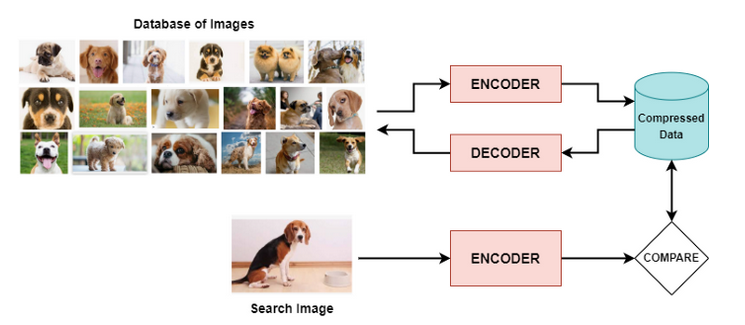
\includegraphics[width=\linewidth]{rys/image_search.png}
	\caption{szukanie obrazów}
	\zrodlo{towards data science}
	\label{fig:image-search}
\end{figure}

\subsubsection{Wykrywanie anomalii}

Innym użytecznym zastosowaniem sieci autoenkoderów jest wykrywanie anomalii. Model wykrywania anomalii można wykorzystać do wykrywania oszukańczych transakcji lub wszelkich zadań nadzorowanych o wysokim stopniu nierównowagi.

Idea polega na trenowaniu autoenkoderów tylko na próbkach danych jednej klasy (klasy większościowej). W ten sposób sieć jest w stanie zrekonstruować dane wejściowe z dobrą lub mniejszą stratą rekonstrukcji. Jeśli przez sieć autoenkodera przepuści się próbkę danych innej klasy docelowej, spowoduje to porównywalnie większą stratę rekonstrukcji.

Można określić wartość progową straty rekonstrukcji (wynik anomalii), której przekroczenie będzie uznawane za anomalię.

\subsubsection{Uzupełnianie brakujących danych}

Do imputacji brakujących wartości w zbiorze danych można wykorzystać autoenkodery odszumiające. Idea polega na trenowaniu sieci autoenkoderów poprzez losowe umieszczanie brakujących wartości w danych wejściowych i próbę odtworzenia oryginalnych danych surowych poprzez minimalizację straty rekonstrukcji.

Po wytrenowaniu wag autoenkodera rekordy zawierające brakujące wartości mogą być przepuszczane przez sieć autoenkodera w celu zrekonstruowania danych wejściowych, także z imputowanymi brakującymi cechami.


\chapter{jakiś tytuł części praktycznej}
%\chapter{Przykłady zastosowań autoenkoderów}

%\section{Analiza PCA za pomocą autoenkodera niedopełnionego}

%Jeśli autoenkoder korzysta jedynie z liniowych funkcji aktywacji, a funkcją kosztu jest  błąd średniokwadratowy (MSE), to będzie on przeprowadzał analizę składowych głównych PCA \cite{geron}. Na rysunku \ref{fig:PCA-kod} widoczny jest kod w języku Python służący do utworzenia takiego autoenkodera, który przeprowadzi analizę PCA na zbiorze trójwymiarowym, rzutując go na przestrzeń dwuwymiarową. Można zauważyć podział autoenkodera na dwie części - enkoder i dekoder. Enkoder przyjmuje dane wejściowe o wymiarze 3, a na wyjściu pojawiają się dane dwuwymiarowe. W przypadku dekodera jest odwrotnie - dane na wejściu są dwuwymiarowe, a na wyjściu trójwymiarowe. Obydwie części są modelami sekwencyjnymi z jedną warstwą gęstą, a cały autoenkoder jest modelem sekwencyjnym, w którym po enkoderze występuje dekoder.

%\begin{figure}[!h]
%	\centering
%	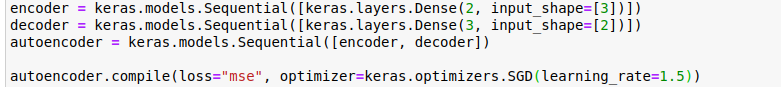
\includegraphics[width=\linewidth]{rys/autoenkoder_PCA_kod.png}
%	\caption{Tworzenie autoenkodera niedopełnionego przeprowadzającego PCA}
%	\zrodlo{Opracowanie własne na podstawie \cite{geron}}
%	\label{fig:PCA-kod}
%\end{figure}

%\begin{figure}[!h]
%	\centering
%	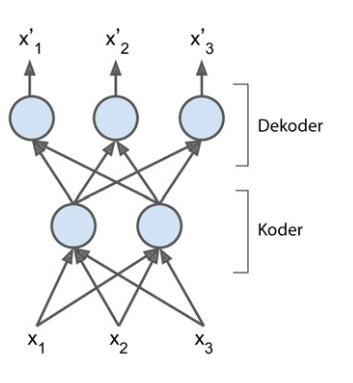
\includegraphics[width=7cm]{rys/ae_undercomplete.png}
%	\caption{Architektura autoenkodera niedopełnionego}
%	\zrodlo{\cite{geron}}
%	\label{fig:ae-undercomplete}
%\end{figure}

%\newpage

%Opisany autoenkoder zostanie wyuczony na wygenerowanym zbiorze trójwymiarowych danych. Warto zwrócić uwagę, że zbiór uczący stanowi jednocześnie dane wejściowe i dane docelowe. Po wytrenowaniu modelu, używamy enkodera do zakodowania danych wejściowych, czyli do zrzutowania ich na przestrzeń dwuwymiarową. Na rysunku \ref{fig:PCA-3d} zaprezentowany jest trójwymiarowy zbiór danych. Rysunek \ref{fig:PCA-2d} przedstawia wynik działania autoenkodera, a więc dane zrzutowane na przestrzeń 2D. Z kolei na rysunku \ref{fig:PCA-zwykle} widoczne jest rzutowanie uzyskane przy użyciu ,,zwykłego'' algorytmu PCA. Na podstawie tych wykresów można stwierdzić, że rzutowanie uzyskane przy pomocy autoenkodera oraz PCA jest takie samo, jedynie układ współrzędnych jest odwrócony o 180 stopni.

%\newpage

%\begin{figure}[!h]
%	\centering
%	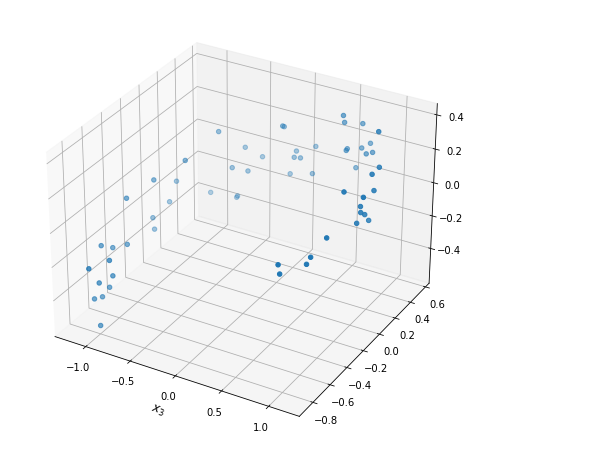
\includegraphics[width=10cm]{rys/pca3d_dane.png}
%	\caption{Wygenerowane dane trójwymiarowe}
%	\zrodlo{Opracowanie własne na podstawie \cite{geron}}
%	\label{fig:PCA-3d}
%\end{figure}


%\begin{figure}[!h]
%	\centering
%	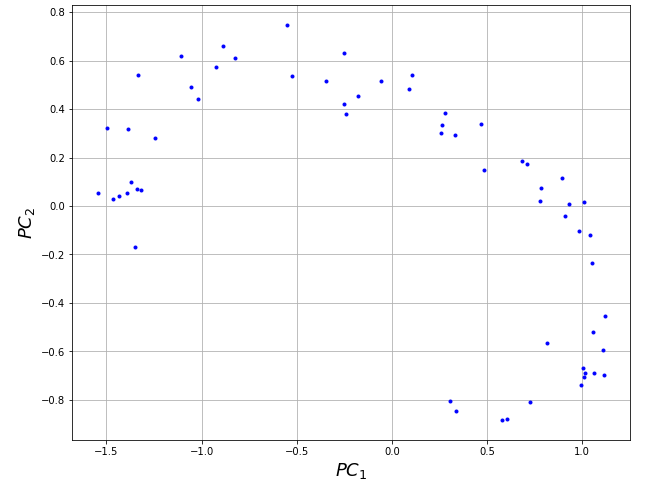
\includegraphics[width=10cm]{rys/pca2d_dane.png}
%	\caption{Rzutowanie dwuwymiarowe przy użyciu autoenkodera, zachowujące maksymalną wariancję}
%	\zrodlo{Opracowanie własne na podstawie \cite{geron}}
%	\label{fig:PCA-2d}
%\end{figure}

%\newpage

%\begin{figure}[!h]
%	\centering
%	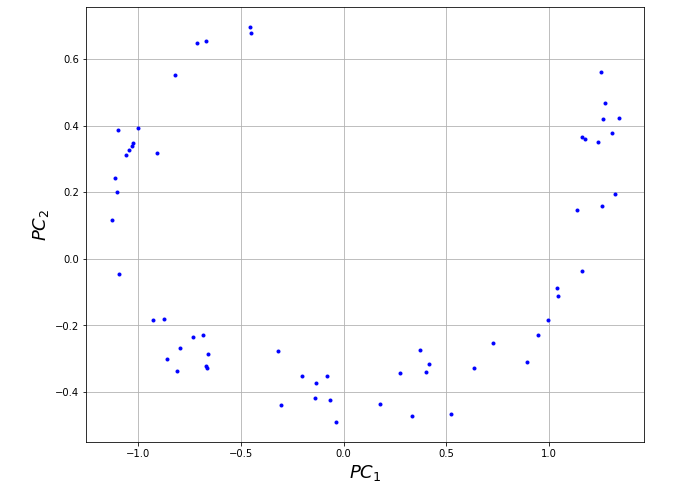
\includegraphics[width=10cm]{rys/pca_zwykle.png}
%	\caption{Rzutowanie dwuwymiarowe przy użyciu PCA, zachowujące maksymalną wariancję}
%	\zrodlo{Opracowanie własne na podstawie \cite{geron}}
%	\label{fig:PCA-zwykle}
%\end{figure}

%\begin{figure}[!h]
%	\centering
%	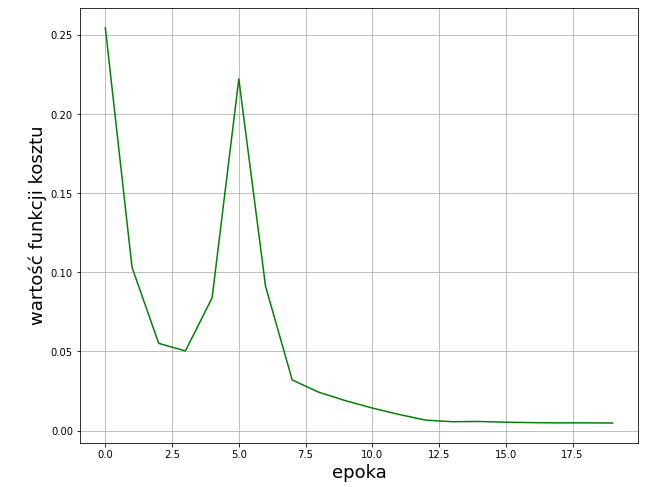
\includegraphics[width=10cm]{rys/ae_undercomplete_loss.png}
%	\caption{Wartość funkcji straty w kolejnych epokach podczas uczenia modelu}
%	\zrodlo{Opracowanie własne}
%	\label{fig:undercomplete-loss}
%\end{figure}

%\section{Kolejny przykład}


\chapter*{Podsumowanie i~wnioski}


\begin{thebibliography}{99}

\bibitem{aggarwal} Aggarwal, C. C. (2018).\emph{ Neural Networks and Deep Learning}, Springer International Publishing

\bibitem{bank} Bank D., Koenigstein N., Giryes R. (2021), \emph{Autoencoders}, arXiv:2003.05991v2

\bibitem{chollet} Chollet F., Allaire J. J. (2019) \emph{Deep Learning. Praca z językiem R i biblioteką Keras}, Helion SA

\bibitem{edureka} Edureka, Autoencoders Tutorial. Autoencoders in Deep Learning. Tensorflow Training \url{https://www.youtube.com/watch?v=nTt_ajul8NY} 

\bibitem{ertel} Ertel W. (2017) \emph{Introduction to Artificial Intelligence. Second Edition}, Springer International Publishing

\bibitem{geron} G\'eron A. (2020) \emph{Uczenie maszynowe z użyciem Scikit-Learn i TensorFlow. Wydanie II}, Helion SA

\bibitem{goodfellow} Goodfellow I., Bengio Y., Courville A. (2018), \emph{Deep Learning. Systemy uczące się}, PWN, Warszawa 

\bibitem{hubel1} Hubel D. H., \emph{Single Unit Activity in  Striate Cortex of Unrestrained Cats}, J. Physiol. (1959) 147, 226-238

\bibitem{hubel2} Hubel D. H., Wiesel T. N., \emph{Receptive Fields of Single Neurones in the Cat's Striate Cortex}, J. Physiol., (1959), 148, 574-591

\bibitem{illustrated} Krohn J., Beyleveld G., Bassens A., \emph{Uczenie głębokie i sztuczna inteligencja. Interaktywny przewodnik ilustrowany}, Helion 2022

\bibitem{kumar} Kumar S., (2021) \emph{7 Applications of Auto-Encoders every Data Scientist  should know. Essential guide to Auto-Encoders and its usage}, Towards Data Science (dostęp: 01.04.2022)

\bibitem{osinga} Osinga D. (2019) \emph{Deep Learning. Receptury}, Helion SA

\bibitem{pinaya} Pinaya W. H. L., Vieira S., Garcia-Dias R., Mechelli A., \emph{Machine Learning. Methods and Applications to Brain Disorders}, Academic Press,
2020

\bibitem{skansi} Skansi S. (2018) \emph{Introduction to Deep Learning. From Logical Calculus to Artificial Intelligence}, Springer International Publishing


\end{thebibliography}



\listoffigures

\listoftables


\chapter*{Załączniki}
\begin{enumerate}
%\item Oświadczenie o oryginalności pracy i możliwości jej wykorzystania. 
%\item Opinia promotora na temat oryginalności pracy oraz w~sprawie dopuszczenia do obrony pracy dyplomowej.
%\item Potwierdzenie analizy antyplagiatowej.
\item Płyta CD z niniejszą pracą w wersji elektronicznej.
\end{enumerate}




\chapter*{Streszczenie (Summary)}

\bigskip
\bigskip

\begin{center}
  \textbf{\tytul}
\end{center}



\bigskip

\begin{center}
  \textbf{\textit{\tytulangielski}}
\end{center}



\selecthyphenation{english}
{\it

}

\end{document}

